\documentclass[12pt, letterpaper]{article}
\usepackage[utf8]{inputenc}
\usepackage{graphicx}
\usepackage{amsmath}
\usepackage{placeins}
\makeatletter
\AtBeginDocument{%
  \expandafter\renewcommand\expandafter\subsection\expandafter
    {\expandafter\@fb@secFB\subsection}%
  \newcommand\@fb@secFB{\FloatBarrier
    \gdef\@fb@afterHHook{\@fb@topbarrier \gdef\@fb@afterHHook{}}}%
  \g@addto@macro\@afterheading{\@fb@afterHHook}%
  \gdef\@fb@afterHHook{}%
}
\makeatother
\makeatletter
\AtBeginDocument{%
  \expandafter\renewcommand\expandafter\subsection\expandafter{%
    \expandafter\@fb@secFB\subsection
  }%
}
\makeatother

\title{Creating a Test Statistic to Find if the Number of Misses in a Song from Guitar Hero is Random}
\author{Shannon Coyle, Samantha Colucci, and Brianna Cirillo}
\date{December 2020}

\begin{document}
\maketitle

\section{INTRODUCTION}
The game, Guitar Hero, collects information regarding the number of “hits” recorded by the player.  This poses the question about the randomness of the misses in a song and if they are correlated to the difficulty of the part of the song.

The study investigates the randomness of different songs using varying methods.  These methods looked at the number of miss streaks over the total number of misses, distances between each miss, and using the runs test.  The resampling of the data sets was performed through parametric bootstrapping, permutation tests, and regular bootstrapping. Using resampling and our methods together allowed us to assess the randomness of a given song based on the results. 

This report explains the methodology used in order to test the randomness of a song. The methods and resampling used throughout the project gave results for the empirical type 1 error and the power of the test. These methods were applied to different songs, therefore, returning different results. This report will also look at the limitations and future ideas for the project, and how some of our methods worked well while others did not.

\section{METHODOLOGY}
\subsection{Method 1}
The first method looks at the proportion of the number of miss streaks over the number of total misses.  A streak was defined as one or more misses in a row since it was easier with the code and some samples did not have that many streaks to look at.  From this method, we discovered that the proportion does not tell us anything about the location of the misses.  This proved to be difficult to determine randomness of misses without knowing the exact location of them.  

\subsection{Method 2}
The second method calculates the distances between misses in a song.  The idea behind this method was that if we can see where the misses are occurring, we can see if they are random.  We can seeing where the distances are occurring randomly and conclude that the misses must also be occurring randomly. 

There was an attempt to use a median distance as a basis rather than the mean because the distances were varied, so the average would not tell us that much.  This led to a problem because a lot of the songs had long miss streaks, which lead to a distance of 0, so the median would also become zero.  With this small issue, it led to the idea of use the runs test on this method and, therefore, the distances.  

\subsection{Runs Test}
Knowing that the runs test is a preconceived test for randomness, the idea behind using this was to use it on the distances of misses within a song, rather than just using it on the song. As mentioned previously if a conclusion can be reached that the distances are random, this would imply randomness of the misses in the song. 

A run is defined as a series of increasing or decreasing values, while the number of values in each series is the length of each run. The number of runs in a data set, denoted R, is crucial because this is the number that is used to derive the test statistic. The other values involved in deriving the test statistics is the expected number of runs, denoted $\bar{R}$, the median value of the data sample, the standard deviation of the number of runs, denoted $s_{R}$, and the number of values below and above the median. 

Once the test statistic is derived, the runs test comes to a conclusion about whether or not to reject the null hypothesis. Here, the test defines: 

$H_{0}$: the sequence is random

$H_{a}$: the sequence is not random

The runs test program used was found from the snpar package in RStudio. A p-value, the number of runs and an alternative hypothesis of nonrandomness is produced once the test is run. This package was specifically chosen because was created to be used on discrete data, rather than continuous. When using this method, each song was resampled and a distance vector for each sample was computed. The runs test was then used on the distances to determine if the null hypothesis of randomness should be rejected or not. 

\subsection{Resampling Methods}
\subsubsection{Parametric Bootstrap}
The Parametric Bootstrap was used to generate a bootstrap using a parameterized distribution.  It takes in a specified number of resamples then performs a Bernoulli distribution in order to resample the data.  The Bernoulli distribution looks at the sample size then the event probability, which was set to $50%$ since the data is composed of 0's and 1's.  This goes through and resamples the data as either a 0 or a 1 for the specified number of resamples that was initialized.   

\subsubsection{Permutation Resampling}
The permutation resampling method is a type of randomization that was developed for data that does not conform to the assumptions needed to perform the statistical method desired. There are multiple advantages to using this type of resampling. In order to implement this, one does not need to know the distribution of the data and it can also be used on small sample sizes. A major disadvantage to using this method is the amount of computer power it takes, since as the sample size begins to increase, the number of permutations computed during the resampling increases rapidly. For this reason, when the permutation resampling is used throughout Methods 1, 2 and the Runs test, the amount of samples produced by this resampling is smaller than that produced by the other resampling techniques.

The main element of this resampling method, that differentiates it from most other methods, is that it resamples *without* replacement. Essentially, it redistributes the original elements of the data in a different order. Though this sampling can be beneficial to use here since the distribution of our data is unknown, it also presents issues when checking for randomness. For example, if there is a detectable pattern in a specific song or sample, the permutation resampling may cause the presence of that pattern to disappear, due to the way the resampling is done. When this became an issue during the research, a different approach was taken to ensure that if the songs being analyzed do have a pattern, that pattern is not lost. This is discussed more in the Power of the Test section. 

\subsubsection{Nonparametric Bootstrap}
Nonparametric bootstrapping is taking a sample of the same size as the data, from the data, but with replacement. This means that even if a data point is resampled, it can be resampled again. The goal of bootstrapping is to approximate the sampling distribution by simulating the data, then using this resamples data as the real data. This allows for data analysis on data that we are not willing to make assumptions about the parameters. On average, the number of times data was bootstrapped was between 200 and 5000 times. 

\section{EMPIRICAL TYPE 1 ERROR AND POWER SIMULATIONS}
To look into the empirical type 1 error rates, random songs were created. In order to create the songs,a sample of 50 observations were taken from a binomial distribution with a probability of 0.5. The songs were resampled using each of the aforementioned methods. The distances of misses in the resampled sample, were then calculated. The runs test was then performed on these distances for each alpha from 0.001 to 0.1 that were incremented at 0.005. This therefore returned the average of the p-values that were less that 0.05 for each theoretical alpha. 

For the final power simulations, different scenarios were used in order to create a song that is not random. This means that the songs created should make the null hypothesis false. Doing this will show how well the metrics identify nonrandomness.The scenarios using positive pairwise correlation generated two songs, one with 200 notes and one with 600 notes. The probability model used was that the probability of missing a note was 0.2 and the correlation between any two consecutive notes was 0.3.The scenarios using blocks with different difficulties also created two songs, one with 200 notes and one with 600 notes. For each song created using this scenario, there were easy, medium, hard, and very hard sections. The probability of missing a note in an easy section is 0.01, in a medium section is 0.05, in a hard section 0.25, and in a very hard section is 0.5. The scenarios using the autoregressive model of order 1 generated six songs, three with 200 notes and three with 600 notes. The probability model used for the first type is the probability of missing a note is 0.1 and the correlation between any two notes is $0.5^{\mid i-j \mid}$. For the probability model for the second type, the probability of missing a note stayed 0.1, but the correlation between any two notes is $0.3^{\mid i-j \mid}$. For the third type, the probability of missing a note is 0.2 and the correlation between any two notes is $0.5^{\mid i-j \mid}$.

\subsection{Parametric Bootstrap}
When resampling with a parametric bootstrap, multiple simulations were run with a varying number of observations - it was usually 50 or 100 observations.  

\subsubsection{Empirical Type 1 Error} 
To calculate the empirical type 1 error rate, the parametric bootstrap worked better with 50 observations as opposed to 100 observations.  There were also two random songs made to see how the error rate varies between songs. These random songs were generated through code in which they were both 50 notes long and had a $50\%$ chance of being a 0 or a 1. Alpha was increased by 0.01, but error rates between 0.005 and 0.001 ended up being 0.00. 
\begin{table}[!h]
\begin{center}
\begin{tabular}{|c|c|c|}
\hline
\textbf{Alpha} & \textbf{Empirical - Random Song 1} & \textbf{Empirical - Random Song 2} \\
\hline
$\alpha = 0.001$ & 0.00 & 0.00\\
$\alpha = 0.005$ &  0.01 & 0.00\\
$\alpha = 0.006$ &  0.01 & 0.02\\
$\alpha = 0.007$ & 0.01 & 0.02\\
$\alpha = 0.008$ & 0.01 & 0.04\\
$\alpha = 0.009$ & 0.01 & 0.04\\
$\alpha = 0.01$ & 0.01 & 0.04\\
$\alpha = 0.02$ & 0.01 & 0.04\\
$\alpha = 0.03$ & 0.01 & 0.06\\
$\alpha = 0.04$ & 0.01 & 0.06\\
$\alpha = 0.05$ &  0.03 & 0.07\\
$\alpha = 0.06$ &  0.06 & 0.08\\
$\alpha = 0.07$ &  0.08 & 0.09\\
$\alpha = 0.08$ &  0.08 & 0.13\\
$\alpha = 0.09$ & 0.08 & 0.13\\
$\alpha = 0.1$ & 0.08 & 0.14\\
\hline
\end{tabular}
\end{center}
\caption{The table above shows the type 1 error rates obtained with their respective alphas.}
\label{fig: Type 1 Error Rates for Parametric Bootstrap}
\end{table}
The table above shows the difference between the two random songs and how the second random song displayed more of a variation of error values.  The second random song showed to have more of a curve and varying error rates, whereas, the first random song had multiple occurrences of the same p-value for different alphas. Refer to figures 1 and 2 in the appendix.

\subsubsection{Final Power Simulations}
When using the Parametric Bootstrap to return a power, they were generally very low p-values or 0.  The power was always equal to 0 when alpha was set to 0.001 and many of the scenarios gave 0 for every value of alpha.  There were three scenarios that gave actual values which were the both blocks methods and the autoregressive model of order 1 that had 200 notes per song, a probability of missing a note as p=0.1, and $\rho = 0.3$. 
\begin{table}[t]
\begin{center}
\begin{tabular}{|c|c|c|c|c|c|}
\hline
\textbf{Type 1 Error Rate Scenario} & $\alpha = 0.001$ &  $\alpha = 0.005$ &  $\alpha = 0.01$ &  $\alpha = 0.05$ &  $\alpha = 0.10$ \\
\hline
Neg. Pair Correlation, n = 200 & 0.00 & 0.00 & 0.00 & 0.00 & 0.00 \\
\hline
Neg. Pair Correlation, n = 600 & 0.00 & 0.00 & 0.00 & 0.00 & 0.00 \\
\hline
Blocks, n = 200 & 0.00 & 0.03 & 0.03 & 0.11 & 0.30 \\
\hline
Blocks, n = 600 & 0.00 & 0.00 & 0.01 & 0.02 & 0.08 \\
\hline
AR(1), p=0.1, $\rho = 0.5$, n = 200 & 0.00 & 0.00 & 0.00 & 0.00 & 0.00 \\
\hline
AR(1), p=0.1, $\rho = 0.5$, n = 600 & 0.00 & 0.00 & 0.00 & 0.00 & 0.00 \\
\hline
AR(1), p=0.1, $\rho = 0.3$, n = 200 & 0.00 & 0.00 & 0.00 & 0.01 & 0.01 \\
\hline
AR(1), p=0.1, $\rho = 0.3$, n = 600 & 0.00 & 0.00 & 0.00 & 0.00 & 0.00 \\
\hline
AR(1), p=0.2, $\rho = 0.5$, n = 200 & 0.00 & 0.00 & 0.00 & 0.00 & 0.00 \\
\hline
AR(1), p=0.2, $\rho = 0.5$, n = 600 & 0.00 & 0.00 & 0.00 & 0.00 & 0.00 \\
\hline
\end{tabular} 
\end{center}
\caption{The table shows the power at each theoretical alpha for each of the scenarios above.}
\label{fig: Power Simulations using Parametric Bootstrap}
\end{table}
From the table, it is evident that most of the values obtained are 0 with exceptions for three of the scenarios.  Aside from the table, the graphs also show the large number of occurrences of 0 as a power. Refer to figures 3 and 4 in the appendix, to see the visualization.

\subsection{Permutation Resampling}
\subsubsection{Empirical Type 1 Error} 
A random song of 50 notes was created by the rbinom() function in Rstudio, which guarantees randomness. This implies that the alpha obtained from the test, the empirical alpha, should project a low rejection rate since the null hypothesis of randomness is known to be true. The resulting random song from this code was:
\begin{gather*}
  0 1 1 1 1 1 1 0 0 0 0 0 0 0 0 1 0 0 0 1 0 
  0 0 0 1 0 1 1 1 1 1 0 0 1 1 1 0 1 0 0 1 1
  1 0 1 0 0 1 1 0
\end{gather*} 
To resample the data, the permutation resampling code was used and the song was resampled 100 times. The runs test was then performed on the distances of misses in each sample. This returned the average of the p-values that were less that 0.05 for each theoretical alpha, this can be seen in the table below.
\begin{table}[h]
\begin{center}
\begin{tabular}{|c|c|}
\textbf{Type 1 Error} & \textbf{Random Song 1}\\
$\alpha = 0.001$ & 0.00\\
$\alpha = 0.005$ &  0.00\\
$\alpha = 0.006$ &  0.00\\
$\alpha = 0.007$ & 0.00\\
$\alpha = 0.008$ & 0.00\\
$\alpha = 0.009$ & 0.01\\
$\alpha = 0.01$ & 0.01\\
$\alpha = 0.02$ & 0.03\\
$\alpha = 0.03$ & 0.05\\
$\alpha = 0.04$ & 0.06\\
$\alpha = 0.05$ &  0.09\\
$\alpha = 0.06$ &  0.09\\
$\alpha = 0.07$ &  0.10\\
$\alpha = 0.08$ &  0.11\\
$\alpha = 0.09$ & 0.11\\
$\alpha = 0.1$ & 0.11 \\
\end{tabular}
\end{center}
\caption{The table above shows the type 1 error rates obtained with their respective alpha.}
\label{fig: Type 1 Error Rates for Permutation Resampling}
\end{table}
The empirical alphas are mostly the same as the theoretical alphas. The empirical alphas, however, do not increase as nicely as the theoretical alphas do, due to how the test performed at each level. For the most part, these empirical alphas match the theoretical alphas. Refer to figure 5, to see the graph.

\subsubsection{Final Power Simulations}
A similar method was used for these power simulations, however once the random song was resampled with the permutation method, 10 different methods were used in order to ensure the test was being used on songs that were nonrandom. This should give us a larger empirical alpha since the null hypothesis is known to be nonrandom. Below is a table of the outcomes of the test run with these 10 different methods.
\begin{table}[h]
\begin{center}
\begin{tabular}{|c|c|c|c|c|c|}
\hline
\textbf{Type 1 Error Rate Scenario} & $\alpha = 0.001$ &  $\alpha = 0.005$ &  $\alpha = 0.01$ &  $\alpha = 0.05$ &  $\alpha = 0.10$ \\
\hline
Neg. Pair Correlation, n = 200 & 0.00 & 0.00 & 0.00 & 0.00 & 0.00 \\
\hline
Neg. Pair Correlation, n = 600 & 0.00 & 0.00 & 0.00 & 0.00 & 0.00 \\
\hline
Blocks, n = 200 & 0.00 & 0.12 & 0.12 & 0.26 & 0.27 \\
\hline
Blocks, n = 600 & 0.00 & 0.08 & 0.09 & 0.16 & 0.27 \\
\hline
AR(1), p=0.1, $\rho = 0.5$, n = 200 & 0.00 & 0.00 & 0.00 & 0.00 & 0.00 \\
\hline
AR(1), p=0.1, $\rho = 0.5$, n = 600 & 0.00 & 0.00 & 0.00 & 0.00 & 0.00 \\
\hline
AR(1), p=0.1, $\rho = 0.3$, n = 200 & 0.01 & 0.01 & 0.01 & 0.01 & 0.01 \\
\hline
AR(1), p=0.1, $\rho = 0.3$, n = 600 & 0.00 & 0.00 & 0.00 & 0.00 & 0.00 \\
\hline
AR(1), p=0.2, $\rho = 0.5$, n = 200 & 0.00 & 0.00 & 0.00 & 0.00 & 0.00 \\
\hline
AR(1), p=0.2, $\rho = 0.5$, n = 600 & 0.00 & 0.00 & 0.00 & 0.00 & 0.00 \\
\hline
\end{tabular}
\end{center}
\caption{The table shows the power at each theoretical alpha for each of the scenarios above.}
\label{fig: Power Simulations using Permutation Resampling}
\end{table}
All of these power values are much lower than desired. They are consistent with previous power tests that were conducted, and all 10 simulations are mostly consistent with each other, however they are not the values that were hoped for. Refer to figure 6 and 7, to see the graph.

\subsection{Nonparametric Bootstrap}
\subsubsection{Empirical Type 1 Error} 
By taking 50 samples from the binomial distribution, the resulting random song was:
\begin{gather*}
  0 1 0 0 0 1 0 0 1 1 0 1 0 1 1 1 1 1 1 1 0 
  1 0 0 1 1 0 0 1 0 0 1 0 0 0 1 0 1 0 1 0 0
  0 1 0 1 1 1 1 0
\end{gather*} 
To resample the data, the nonparametric bootstrap was used and the song was resampled 100 times. The runs test was then performed on the distances of misses in the bootstrapped sample. This returned the average of the p-values that were less that 0.05 for each theoretical alpha, which can be seen in the table below.

\begin{table}[hb]
\begin{center}
\begin{tabular}{|c|c|}
\textbf{Type 1 Error} & \textbf{Random Song 1}\\
$\alpha = 0.001$ & 0.00\\
$\alpha = 0.005$ &  0.00\\
$\alpha = 0.006$ &  0.00\\
$\alpha = 0.007$ & 0.00\\
$\alpha = 0.008$ & 0.02\\
$\alpha = 0.009$ & 0.02\\
$\alpha = 0.01$ & 0.02\\
$\alpha = 0.02$ & 0.03\\
$\alpha = 0.03$ & 0.03\\
$\alpha = 0.04$ & 0.05\\
$\alpha = 0.05$ &  0.05\\
$\alpha = 0.06$ &  0.05\\
$\alpha = 0.07$ &  0.05\\
$\alpha = 0.08$ &  0.06\\
$\alpha = 0.09$ & 0.07\\
$\alpha = 0.1$ & 0.08 \\ 
\end{tabular}
\end{center}
\caption{A function was created to loop through p-values from 0.001 to 0.1 that incremented by 0.005, in order to  generate the Type 1 Error Rates. The table above shows the rates obtained with their respective alpha.}
\label{fig: Type 1 Error Rates for Nonparametric Bootstrap}
\end{table}
The empirical alpha seems to very roughly, match the theoretical alphas. Although, the empirical alphas were not increasing consistently. They would get stuck at certain alphas such as 0.02 and 0.05. Therefore, the theoretical alphas are increasing at a faster rate than the empirical alphas are. Refer to figure 8 to see the plot.

\subsubsection{Final Power Simulations}
For the final power simulations, the majority of the scenarios gave a power of 0. This is extremely low, but overall pretty consistent with our previous findings. The blocks scenario, when the song had 200 notes, gave errors of 0.04 for alphas equal to 0.005, 0.01, 0.05, and 0.10. When the song had 600 notes, the error rates were 0.01 for alphas equal to 0.005, 0.01, 0.05, and 0.10. This potentially means that the runs test on the distance of misses detected nonrandomness more in the block scenarios. In the autocorrelation scenario with 200 notes, where the probability of missing a note was 0.1, and the correlation between any two notes was $0.3^{\mid i-j \mid}$, when alpha was 0.05 and 0.10, the error was 0.01. This could mean that when alpha is 0.05 and 0.10 in this scenario of autocorrelation, that nonrandomness was detected more. In the autocorrelation scenario with 600 notes, where the probability of missing a note was 0.2, and the correlation between any two notes was $0.5^{\mid i-j \mid}$, when alpha was 0.005, 0.01, 0.05, and 0.10 the error was 0.01. Therefore, the detection of nonrandomness was higher in this scenario. This is shown in the table below and figures 9-12 in the appendix.
\begin{table}[h]
\begin{center}
\begin{tabular}{|c|c|c|c|c|c|}
\hline
\textbf{Type 1 Error Rate Scenario} & $\alpha = 0.001$ &  $\alpha = 0.005$ &  $\alpha = 0.01$ &  $\alpha = 0.05$ &  $\alpha = 0.10$ \\
\hline
Neg. Pair Correlation, n = 200 & 0.00 & 0.00 & 0.00 & 0.00 & 0.00 \\
\hline
Neg. Pair Correlation, n = 600 & 0.00 & 0.00 & 0.00 & 0.00 & 0.00 \\
\hline
Blocks, n = 200 & 0.00 & 0.04 & 0.04 & 0.04 & 0.04 \\
\hline
Blocks, n = 600 & 0.00 & 0.01 & 0.01 & 0.01 & 0.01 \\
\hline
AR(1), p=0.1, $\rho = 0.5$, n = 200 & 0.00 & 0.00 & 0.00 & 0.00 & 0.00 \\
\hline
AR(1), p=0.1, $\rho = 0.5$, n = 600 & 0.00 & 0.00 & 0.00 & 0.00 & 0.00 \\
\hline
AR(1), p=0.1, $\rho = 0.3$, n = 200 & 0.00 & 0.00 & 0.00 & 0.01 & 0.01 \\
\hline
AR(1), p=0.1, $\rho = 0.3$, n = 600 & 0.00 & 0.00 & 0.00 & 0.00 & 0.00 \\
\hline
AR(1), p=0.2, $\rho = 0.5$, n = 200 & 0.00 & 0.00 & 0.00 & 0.00 & 0.00 \\
\hline
AR(1), p=0.2, $\rho = 0.5$, n = 600 & 0.00 & 0.01 & 0.01 & 0.01 & 0.01 \\
\hline
\end{tabular}
\end{center}
\caption{The table shows the power at each theoretical alpha for each of the scenarios above.}
\label{fig: Power Simulations using Nonparametric Bootstrap}
\end{table}

\section{APPLICATION}
The hits and misses data was collected on seven songs: "Judith", "Hurts", "American Girl", "Funky", "Ring of Fire", "Watchtower", and "Wolf". For each of these songs, the methods explained above were used to determine if the hits and misses were random. Since method 2 calculates the distances between misses, which was used for the runs test calculations, method 2 was not tested on its own. Therefore, method 1 and the runs test on the distances between misses were calculated for each song using the three different resampling methods.

To obtain a p-value for each song, 100 bootstraps were performed to change the 0's and 1's to different orders and sequences.  Previously, 1000 bootstraps were being done, but it was taking a significant amount of time to return a p-value.  The null hypothesis being followed is that the songs are random and the alternative hypothesis is that the songs are not random. A significance level of $\alpha$ = 0.05 is being used. The results we have here are based solely off of the p-values obtained from these results. Confidence intervals would be a way to improve the strength of these results, which is discussed more in the Future Research section of this paper.

\subsubsection{Parametric Bootstrap}
The p-value of the Method 1 test tells us to reject the null hypothesis while the Run tests p-value tells us to fail to reject the null hypothesis.
\begin{table}[h]
\begin{center}
\begin{tabular}{|c|c|c|}
\hline
\textbf{Method Type} & P-Value \\
\hline
Method 1 & 0 \\
\hline
Runs Test & 0.512 \\ 
\hline
\end{tabular} 
\end{center}
\caption{The table shows the resulting p-values of the method 1 and runs test on the song, "Judith".}
\label{fig: P-values for "Judith": Parametric Bootstrap}
\end{table}

\subsubsection{Permutation Resampling}
Using just these p-values, we would reject the null hypothesis of randomness using Method 1, however fail to reject the null hypothesis when using the runs test on the distances. This implies that we may come to two different conclusions about the randomness of the songs depending on which method we are using. 
\begin{table}[h]
\begin{center}
\begin{tabular}{|c|c|c|}
\hline
\textbf{Method Type} & P-Value \\
\hline
Method 1 & 0 \\
\hline
Runs Test & 0.847 \\ 
\hline
\end{tabular}
\end{center}
\caption{The table shows the resulting p-values of the method 1 and runs test on the song, "Judith".}
\label{fig: P-values for "Judith": Permutation Resampling}
\end{table}

\subsubsection{Nonparametric Bootstrap}
The nonparametric bootstrap was used to resample the song "Judith", in order to test for randomness using method 1 and the runs test. The resulting p-values for each of the tests can be seen in the table below. After the song bootstrapped 1000 times, the statistic for method 1 was calculated, the proportion of the number of miss streaks over the number of total misses. This resulted in a p-value of 0. The null hypothesis for method 1 is randomness, thus we would reject the null at the level 0.05. Therefore, we cannot conclude that the song, "Judith" is random. 

To find the test statistic for the runs test, "Judith" was bootstrapped 100 times, the distances between misses was calculates, and the runs test was ran on the distances. This resulted in a p-value of 0.998. The null hypothesis of the runs test is that the data is normal. Since we fail to reject the null at the level 0.05, we do not have enough evidence to conclude that the data is not random.
\begin{table}[h]
\begin{center}
\begin{tabular}{|c|c|c|}
\hline
\textbf{Method Type} & P-Value \\
\hline
Method 1 & 0 \\
\hline
Runs Test & 0.998 \\ 
\hline
\end{tabular}
\end{center}
\caption{The table shows the resulting p-values of the method 1 and runs test on the song, "Judith".}
\label{fig: P-values for "Judith": Nonparametric Bootstrap}
\end{table}

\subsection{Song 2: "Hurts"}
\subsubsection{Parametric Bootstrap}
The p-value of the Method 1 test tells us to reject the null hypothesis while the Run tests p-value tells us to fail to reject the null hypothesis.
\begin{table}[h]
\begin{center}
\begin{tabular}{|c|c|c|}
\hline
\textbf{Method Type} & P-Value \\
\hline
Method 1 & 0  \\
\hline
Runs Test & 0.512 \\ 
\hline
\end{tabular} 
\end{center}
\caption{The table shows the resulting p-values of the method 1 and runs test on the song, "Hurts".}
\label{fig: P-values for "Hurts": Parametric Bootstrap}
\end{table}

\subsubsection{Permutation Resampling}
According to the p-value of the Method 1 test, the null hypothesis would be rejected, meaning there is enough evidence to say that the songs are not random. However, according to the p-value obtained from the Runs Test, we would fail to reject the null hypothesis of randomness. Similarly to the test done on the song "Judith" with permutation resampling, these are contrasting results.
\begin{table}[h]
\begin{center}
\begin{tabular}{|c|c|c|}
\hline
\textbf{Method Type} & P-Value \\
\hline
Method 1 & 0  \\
\hline
Runs Test & 0.249 \\ 
\hline
\end{tabular}
\end{center}
\caption{The table shows the resulting p-values of the method 1 and runs test on the song, "Hurts".}
\label{fig: P-values for "Hurts":Permutation Resampling}
\end{table}

\subsubsection{Nonparametric Bootstrap}
For the song, "Hurts", the nonparametric bootstrap was used to resample the song in order to test for randomness using method 1 and the runs test. The resulting p-values for each of the tests can be seen in the table below. The song was bootstrapped 1000 times and the test statistic for method 1 was calculated. The resulting p-value was 0.186. Thus we would fail to reject the null at the level 0.05. Therefore, we can conclude that the song, "Hurts" is random. 

For the runs test, "Hurts" was bootstrapped 100 times. The runs test was ran on the distances from the bootstrapped sample, which resulted in a p-value of 0.459. Therefore, we fail to reject the null at the level 0.05. We do not have enough evidence to conclude that the song, "Hurts", is not random.
\begin{table}[h]
\begin{center}
\begin{tabular}{|c|c|c|}
\hline
\textbf{Method Type} & P-Value \\
\hline
Method 1 & 0.186  \\
\hline
Runs Test & 0.459 \\ 
\hline
\end{tabular}
\end{center}
\caption{The table shows the resulting p-values of the method 1 and runs test on the song, "Hurts".}
\label{fig: P-values for "Hurts": Nonparametric Bootstrap}
\end{table}

\subsection{Song 3: "American Girl"}
\subsubsection{Parametric Bootstrap}
The p-value of the Method 1 test tells us to fail to reject the null hypothesis and the Run tests p-value tells us to fail to reject the null hypothesis as well.
\begin{table}[h]
\begin{center}
\begin{tabular}{|c|c|}
\hline
\textbf{Method Type} & P-Value \\
\hline
Method 1 & 0.16 \\
\hline
Runs Test & 0.211 \\ 
\hline 
\end{tabular} 
\end{center}
\caption{The table shows the resulting p-values of the method 1 and runs test on the song, "American Girl".}
\label{fig: P-values for "American Girl": Parametric Bootstrap}
\end{table}

\subsubsection{Permutation Resampling}
These p-values alone give us contrasting results once again. The Method 1 test p-value implies that the null hypothesis of randomness would be rejected, while the Runs Test p-value says that we should fail to reject the null hypothesis. 
\begin{table}[h]
\begin{center}
\begin{tabular}{|c|c|c|}
\hline
\textbf{Method Type} & P-Value \\
\hline
Method 1 & 0  \\
\hline
Runs Test & 0.414 \\ 
\hline
\end{tabular}
\end{center}
\caption{The table shows the resulting p-values of the method 1 and runs test on the song, "American Girl".}
\label{fig: P-values for "American Girl": Permutation Resampling}
\end{table}

\subsubsection{Nonparametric Bootstrap}
In order to test for randomness using method 1 and the runs test, "American Girl" was bootstrapped 1000 times. This resulted in p-values for each of the tests, which can be seen in the table below. "American Girl" was bootstrapped 1000 times and the test statistic for method 1 was calculated. The resulting p-value was 0. Hence, we would reject the null at the level 0.05. Therefore, we cannot conclude that the song, "American Girl" is random. 

"American Girl" was bootstrapped 100 times for the runs test. The bootstrapped sample was used to calculate the test statistic for the run's test, which resulted in a p-value of 0.841. Thus, we fail to reject the null at the level 0.05. We do not have enough evidence to conclude that the song, "American Girl", is not random.
\begin{table}[h]
\begin{center}
\begin{tabular}{|c|c|c|}
\hline
\textbf{Method Type} & P-Value \\
\hline
Method 1 & 0  \\
\hline
Runs Test & 0.841 \\ 
\hline
\end{tabular}
\end{center}
\caption{The table shows the resulting p-values of the method 1 and runs test on the song, "American Girl".}
\label{fig: P-values for "American Girl": Nonparametric Bootstrap}
\end{table}

\subsection{Song 4: "Funky"}
\subsubsection{Parametric Bootstrap}
The p-value of the Method 1 test tells us to reject the null hypothesis while the Run tests p-value tells us to fail to reject the null hypothesis.
\begin{table}[h]
\begin{center}
\begin{tabular}{|c|c|c|}
\hline
\textbf{Method Type} & P-Value \\
\hline
Method 1 & 0 \\
\hline
Runs Test & 0.08  \\ 
\hline
\end{tabular} 
\end{center}
\caption{The table shows the resulting p-values of the method 1 and runs test on the song, "Funky".}
\label{fig: P-values for "Funky": Parametric Bootstrap}
\end{table}

\subsubsection{Permutation Resampling}
These p-values are very similar to those of the tests on "American Girl" using permutation resampling. Rejecting the null hypothesis for the Method 1 test and failing to reject the null hypothesis for the Runs test leaves us with conflicting results since both tests have a null hypothesis of randomness. 
\begin{table}[h]
\begin{center}
\begin{tabular}{|c|c|c|}
\hline
\textbf{Method Type} & P-Value \\
\hline
Method 1 & 0 \\
\hline
Runs Test & 0.442  \\ 
\hline
\end{tabular}
\end{center}
\caption{The table shows the resulting p-values of the method 1 and runs test on the song, "Funky".}
\label{fig: P-values for "Funky": Permutation Resampling}
\end{table}

\subsubsection{Nonparametric Bootstrap}
The resulting in p-values for method 1 and the runs test, can be seen in the table below. "Funky" was bootstrapped 1000 times and the test statistic for method 1 was calculated, for which the p-value was 0. Hence, we would reject the null at the level 0.05. Therefore, we cannot conclude that the song, "Funky" is random. 

The test statistic for the runs test for "Funky" was calculated after the song was bootstrapped 100 times. The p-value of the test is 0.656. We fail to reject the null at the level 0.05. We do not have enough evidence to conclude that the song, "Funky", is not random.
\begin{table}[h]
\begin{center}
\begin{tabular}{|c|c|c|}
\hline
\textbf{Method Type} & P-Value \\
\hline
Method 1 & 0  \\
\hline
Runs Test & 0.656 \\ 
\hline
\end{tabular}
\end{center}
\caption{The table shows the resulting p-values of the method 1 and runs test on the song, "Funky".}
\label{fig: P-values for "Funky": Nonparametric Bootstrap}
\end{table}

\subsection{Song 5: "Ring of Fire"}
\subsubsection{Parametric Bootstrap}
The p-value of the Method 1 test tells us to reject the null hypothesis while the Run tests p-value tells us to fail to reject the null hypothesis.
\begin{table}[h]
\begin{center}
\begin{tabular}{|c|c|c|}
\hline
\textbf{Method Type} & P-Value  \\
\hline
Method 1 & 2.204 $[e^{-16}]$ \\
\hline
Runs Test & 0.44 \\ 
\hline
\end{tabular}
\end{center}
\caption{The table shows the resulting p-values of the method 1 and runs test on the song, "Ring of Fire".}
\label{fig: P-values for "Ring of Fire": Parametric Bootstrap}
\end{table}

\subsubsection{Permutation Resampling}
Similarly to the other results of the hypothesis tests with permutation resampling, we have differing results here. The p-value of the Method 1 test tells us to reject the null hypothesis while the Run tests p-value tells us to fail to reject the null hypothesis.
\begin{table}[h]
\begin{center}
\begin{tabular}{|c|c|c|}
\hline
\textbf{Method Type} & P-Value  \\
\hline
Method 1 & 2.204 $[e^{-16}]$ \\
\hline
Runs Test & 0.614 \\ 
\hline
\end{tabular}
\end{center}
\caption{The table shows the resulting p-values of the method 1 and runs test on the song, "Ring of Fire".}
\label{fig: P-values for "Ring of Fire": Permutation Resampling}
\end{table}

\subsubsection{Nonparametric Bootstrap}
The p-values for method 1 and the runs test, can be seen in the table below. "Ring of Fire" was bootstrapped 1000 times and the test statistic for method 1 was calculated. The resulting p-value was approximately 0. We would reject the null at the level 0.05. Thus, we cannot conclude that the song, "Ring of Fire" is random. 

"Ring of Fire" was bootstrapped 100 times and the test statistic for the runs test was calculated. The p-value of the test is 0.317. We fail to reject the null at the level 0.05. We do not have enough evidence to conclude that the song, "Ring of Fire", is not random.
\begin{table}[h]
\begin{center}
\begin{tabular}{|c|c|c|}
\hline
\textbf{Method Type} & P-Value \\
\hline
Method 1 & 0  \\
\hline
Runs Test & 0.317 \\ 
\hline
\end{tabular}
\end{center}
\caption{The table shows the resulting p-values of the method 1 and runs test on the song, "Ring of Fire".}
\label{fig: P-values for "Ring of Fire": Nonparametric Bootstrap}
\end{table}

\subsection{Song 6: "Watchtower"}
\subsubsection{Parametric Bootstrap}
The p-value of the Method 1 test tells us to reject the null hypothesis while the Run tests p-value tells us to fail to reject the null hypothesis.
\begin{table}[h]
\begin{center}
\begin{tabular}{|c|c|c|}
\hline
\textbf{Method Type} & P-Value  \\
\hline
Method 1 & 2.204 $[e^{-16}]$ \\
\hline
Runs Test & 0.66 \\ 
\hline
\end{tabular}
\end{center}
\caption{The table shows the resulting p-values of the method 1 and runs test on the song, "Watchtower".}
\label{fig: P-values for "Watchtower": Parametric Bootstrap}
\end{table}

\subsubsection{Permutation Resampling}
Here, the Method 1 test says to reject the null hypothesis of randomness and the Runs test says to fail to reject the null hypothesis.
\begin{table}[h]
\begin{center}
\begin{tabular}{|c|c|c|}
\hline
\textbf{Method Type} & P-Value  \\
\hline
Method 1 & 2.204 $[e^{-16}]$ \\
\hline
Runs Test & 0.577 \\ 
\hline
\end{tabular}
\end{center}
\caption{The table shows the resulting p-values of the method 1 and runs test on the song, "Watchtower".}
\label{fig: P-values for "Watchtower": Permutation Resampling}
\end{table}

\subsubsection{Nonparametric Bootstrap}
The p-values for method 1 and the runs test, can be seen in the table below. "Watchtower" was bootstrapped 1000 times and the test statistic for method 1 was calculated. The resulting p-value was approximately 0. We would reject the null at the level 0.05. Hence, we cannot conclude that the song, "Watchtower" is random. 

The test statistic for the runs test was calculated after "Watchtower" was bootstrapped 100 times. The p-value of the test is 0.727. We fail to reject the null at the level 0.05. We do not have enough evidence to conclude that the song, "Watchtower", is not random.
\begin{table}[h]
\begin{center}
\begin{tabular}{|c|c|c|}
\hline
\textbf{Method Type} & P-Value \\
\hline
Method 1 & 0  \\
\hline
Runs Test & 0.727 \\ 
\hline
\end{tabular}
\end{center}
\caption{The table shows the resulting p-values of the method 1 and runs test on the song, "Watchtower".}
\label{fig: P-values for "Watchtower": Nonparametric Bootstrap}
\end{table}

\subsection{Song 7: "Wolf"}
\subsubsection{Parametric Bootstrap}
The Method 1 test says to reject the null hypothesis of randomness and the Runs test says to fail to reject the null hypothesis.
\begin{table}[!h]
\begin{center}
\begin{tabular}{|c|c|c|}
\hline
\textbf{Method Type} & P-Value  \\
\hline
Method 1 & 2.204 $[e^{-16}]$ \\
\hline
Runs Test & 0.58 \\ 
\hline
\end{tabular}
\end{center}
\caption{The table shows the resulting p-values of the method 1 and runs test on the song, "Wolf".}
\label{fig: P-values for "Wolf": Parametric Bootstrap}
\end{table}

\subsubsection{Permutation Resampling}
Similar to all of the other results in this section for permutation resampling, these p-values are telling us to do two different things. The p-value of the Method 1 test is telling us to reject the null hypothesis while the p-value of the Runs test is telling us to fail to rejcet the null hypothesis. Since these results are all differing, we cannot make a definite conclusion on whether there is enough evidence to conclude that these songs are random.
\begin{table}[h]
\begin{center}
\begin{tabular}{|c|c|c|}
\hline
\textbf{Method Type} & P-Value  \\
\hline
Method 1 & 0.06 \\
\hline
Runs Test & 0.265 \\ 
\hline
\end{tabular}
\end{center}
\caption{The table shows the resulting p-values of the method 1 and runs test on the song, "Wolf".}
\label{fig: P-values for "Wolf": Permutation Resampling}
\end{table}

\subsubsection{Nonparametric Bootstrap}
The p-values for method 1 and the runs test, can be seen in the table below. The test statistic for method 1 was calculated after "Wolf" was bootstrapped 1000 times. The resulting p-value was 0.02. We would reject the null at the level 0.05. Hence, we cannot conclude that the song, "Wolf" is random. 

The test statistic for the runs test was calculated after "Wolf" was bootstrapped 100 times. The p-value resulting from the test is 0.727. We fail to reject the null at the level 0.05. We do not have enough evidence to conclude that the song, "Wolf", is not random.
\begin{table}[!h]
\begin{center}
\begin{tabular}{|c|c|c|}
\hline
\textbf{Method Type} & P-Value \\
\hline
Method 1 & 0.02  \\
\hline
Runs Test & 0.727 \\ 
\hline
\end{tabular}
\end{center}
\caption{The table shows the resulting p-values of the method 1 and runs test on the song, "Wolf".}
\label{fig: P-values for "Wolf": Nonparametric Bootstrap}
\end{table}

\section{DISCUSSION/LIMITATIONS/IDEAS FOR FURTHER RESEARCH}
\subsection{Discussion}
Overall, the tests conducted on this data were mostly inconclusive. Many of the p-values obtained led us to little to no conclusions. This however, is beneficial in a way because we made progress towards how our methods need to be modified and how they could possibly be used in the future. Due to the following limitations we were unable to obtain as many results as we had hoped, however in the Future Research section below we discuss what couldbe done to help move past these limitations and hopefully provide further results.

\subsections{Limitations}
One of the main limitations that we ran into durig this research was the extent of what we could find out about the runs test. Since the runs test that was implemented was taken from an Rstudio package, it did not give all of the information desired about the runs test statistic, how the number of runs was calculated, and more. Though we were able to figure most of these things out, we could not derive exactly how the runs test statistic was calculated since there are different methods to compute this, depending on which form of the runs test being used. Knowing how this test statistic is computed and being able to view this in addition ot the p-value of the test would give more flexibility in what we could do with our results.

\subsection{Ideas for Future Research}
To continue this research, some additional things can be done. Looking into splitting the song into sections before using these tests could help determine randomness in a different way. This may also give more information on how the level of difficulty varies throughout the song, since it would be visible which specific parts of the song are random and which are not. Multiple plays of the same song may also help since there would be more data to work with and comparisons could be made between the resamplings of the different plays.

In addition, a new method to look into would be the Serial Method. This method counts the number of "01"s together in a song.  From this method, it can be concluded that the larger number of 01s meant that there is a larger number of hits turned into misses.  The possible idea once the method works as anticipated is to compare the number of 01s for each individual row of a bootstrap to the total number of 01s in the entire bootstrap.

In addition to p-values, our results may have been stronger if confidence intervals were included. This was difficult to do because of the limitations of our knowledge on the runs test statistic. However, in the future, creating confidence intervals for the tests once the runs test statistic is obtained would give the ability to come to better conclusions of the tests.

\section{APPENDIX}
\begin{figure}[!hb]
\centering
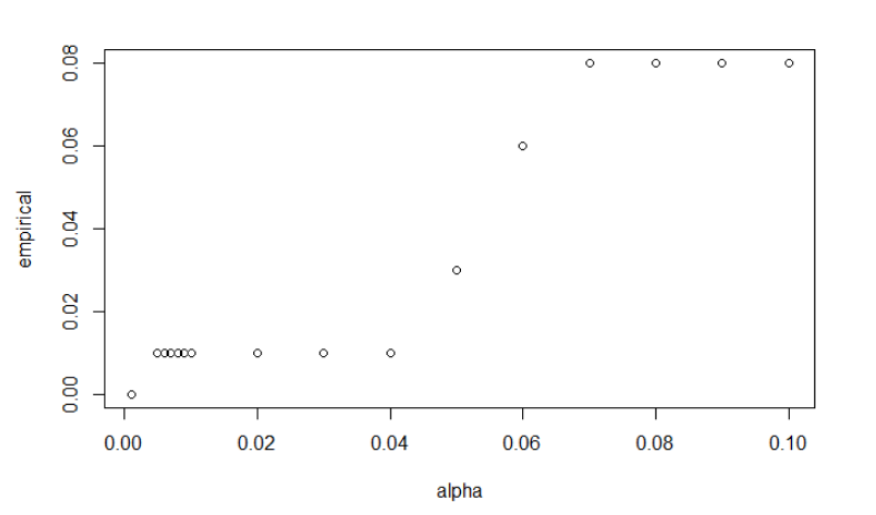
\includegraphics[width=10cm]{Type1_Song1.png}
\caption{Graph of Type 1 error rates for Random Song 1 with 50 observations}
\label{fig: Type 1 Error, Song 1, n=50}
\end{figure}

\begin{figure}[!hb]
\centering
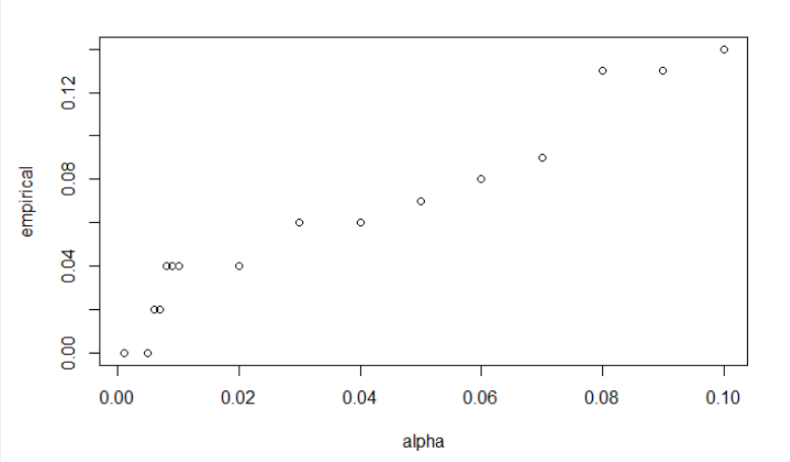
\includegraphics[width=10cm]{Type1_Song2.png}
\caption{Graph of Type 1 error rates for Random Song 2 with 50 observations}
\label{fig: Type 1 Error, Song 2, n=50}
\end{figure}

\begin{figure}[!hb]
\centering
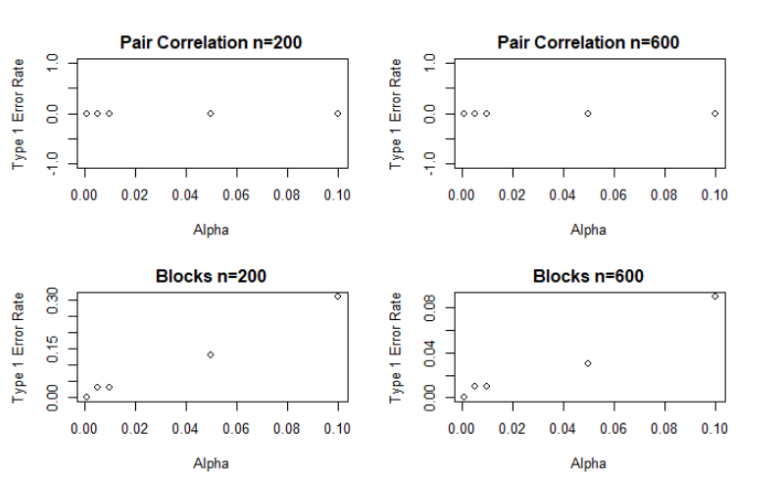
\includegraphics[width=10cm]{PowerGraphs1.png}
\caption{Graph of first four scenarios to calculate the power of a test}
\label{fig: Power Graphs 1}
\end{figure}

\begin{figure}[!hb]
\centering
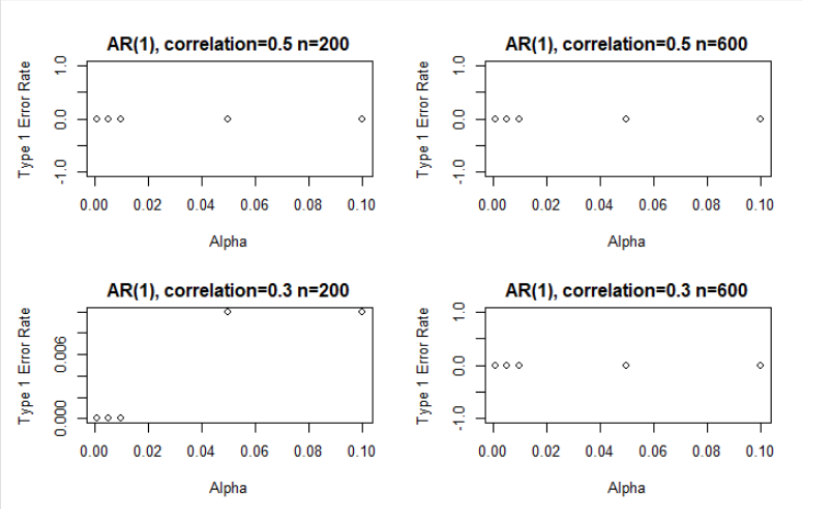
\includegraphics[width=10cm]{PowerGraphs2.png}
\caption{Graph of last four scenarios to calculate the power of a test}
\label{fig: Power Graphs 2}
\end{figure}

\begin{figure}[!hb]
\centering
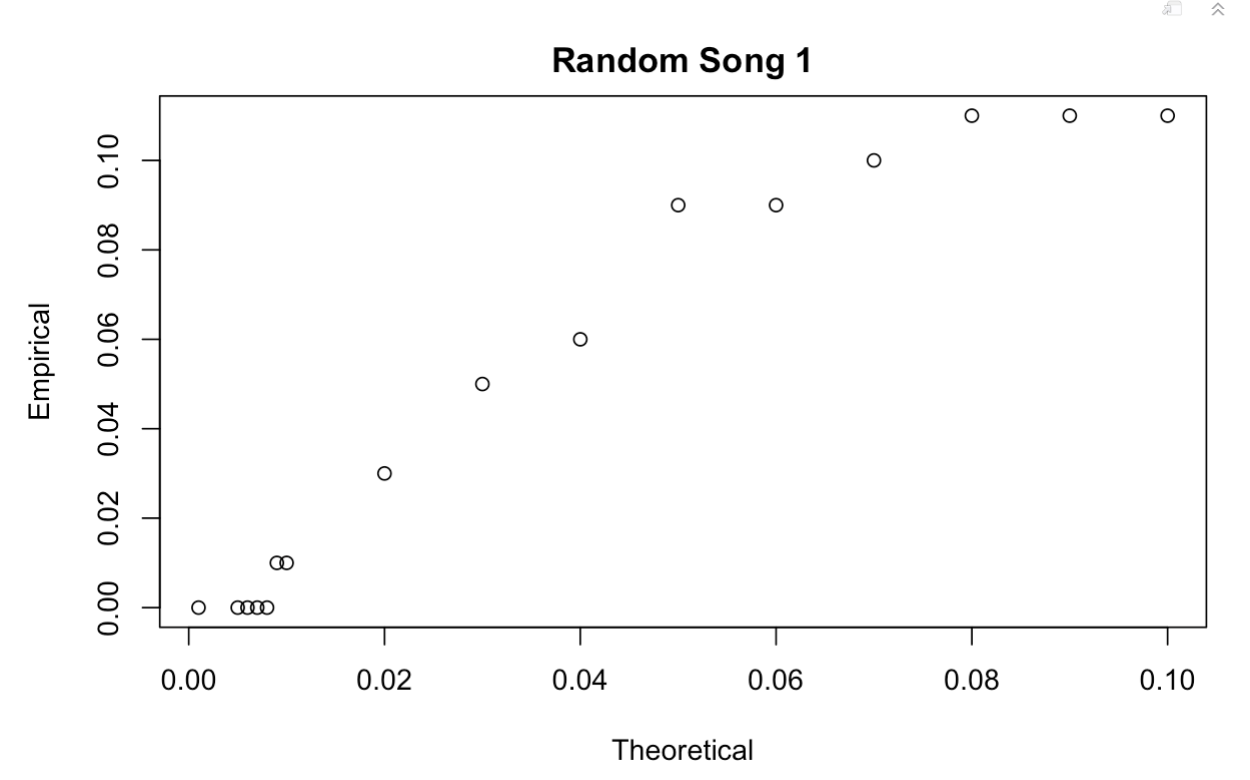
\includegraphics[width=10cm]{EmpiricalvsTheoreticalAlpha.png}
\caption{Graph of Type 1 error rates with 50 observations}
\label{fig: Type 1 Error, n=50}
\end{figure}

\begin{figure}[!hb]
\centering
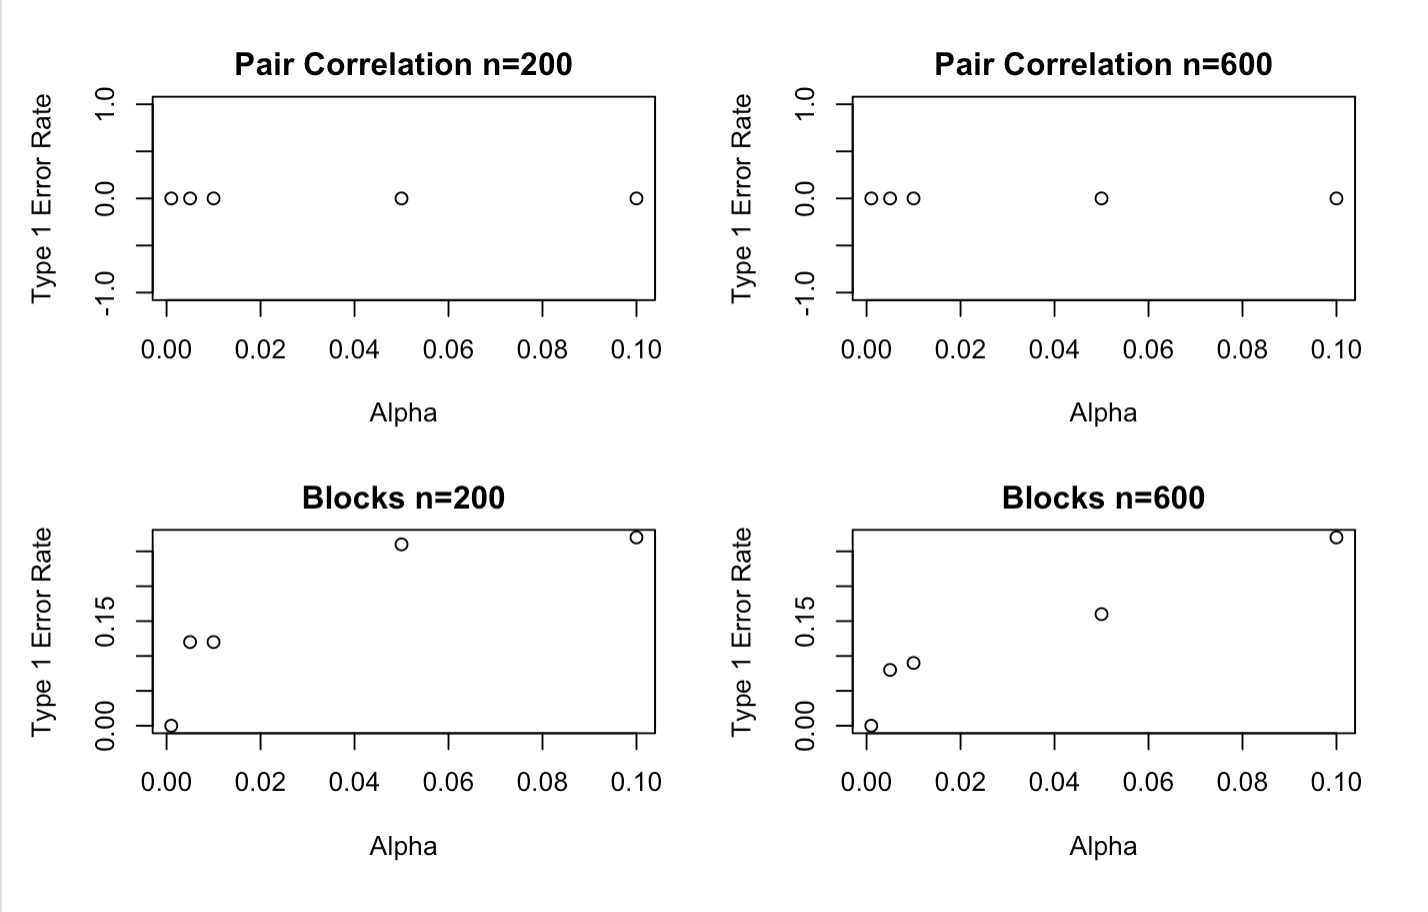
\includegraphics[width=10cm]{Blocks&PairCorrelation.png}
\caption{Graph of first four scenarios to calculate the power of a test}
\label{fig: Power Graphs 1}
\end{figure}

\begin{figure}[!hb]
\centering
\includegraphics[width=10cm]{AR_correlationPlots.png}
\caption{Graph of last four scenarios to calculate the power of a test}
\label{fig: Power Graphs 2}
\end{figure}

\begin{figure}[!hb]
\centering
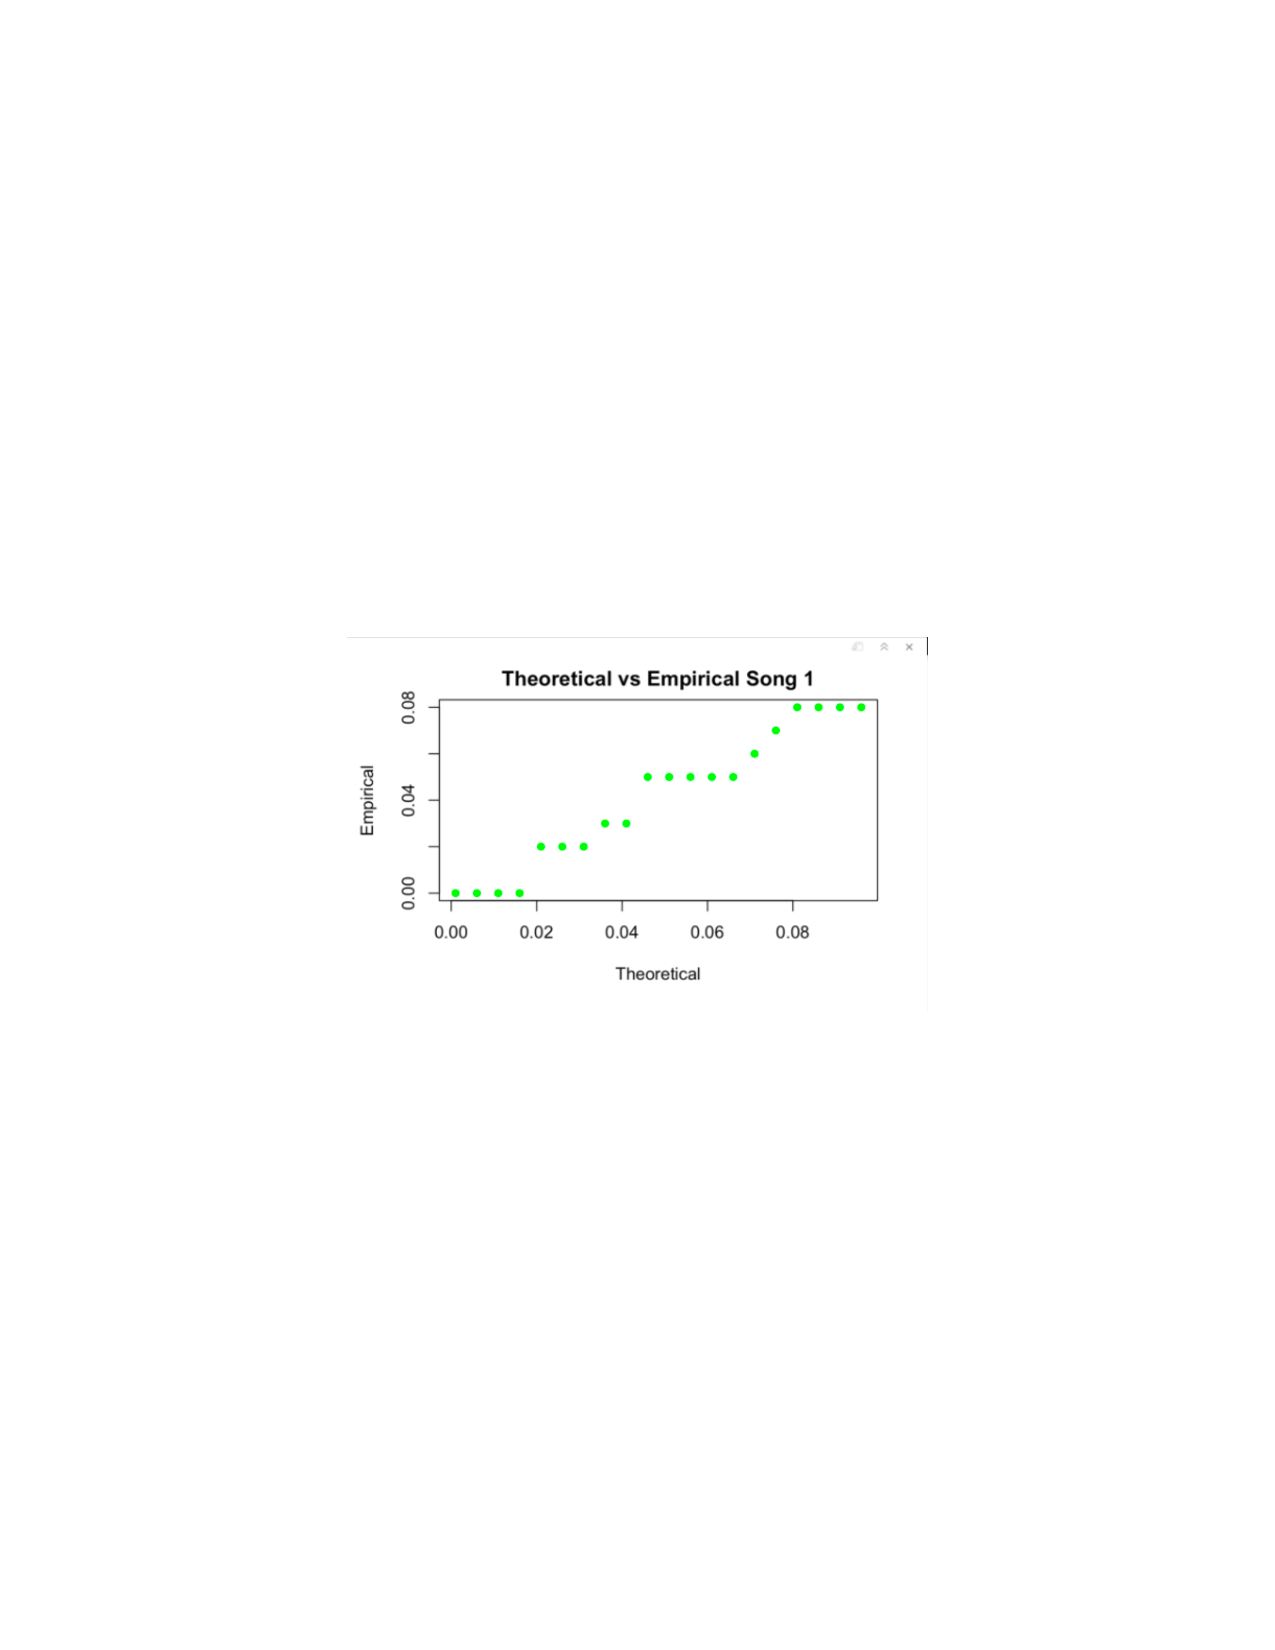
\includegraphics[width=10cm]{PowerGraph_nonparamboot.pdf}
\caption{Graph of Type 1 error rates for Random Song 1 with 50 observations}
\label{fig: Type 1 Error, Song 1, n=50}
\end{figure}

\begin{figure}[!hb]
\centering
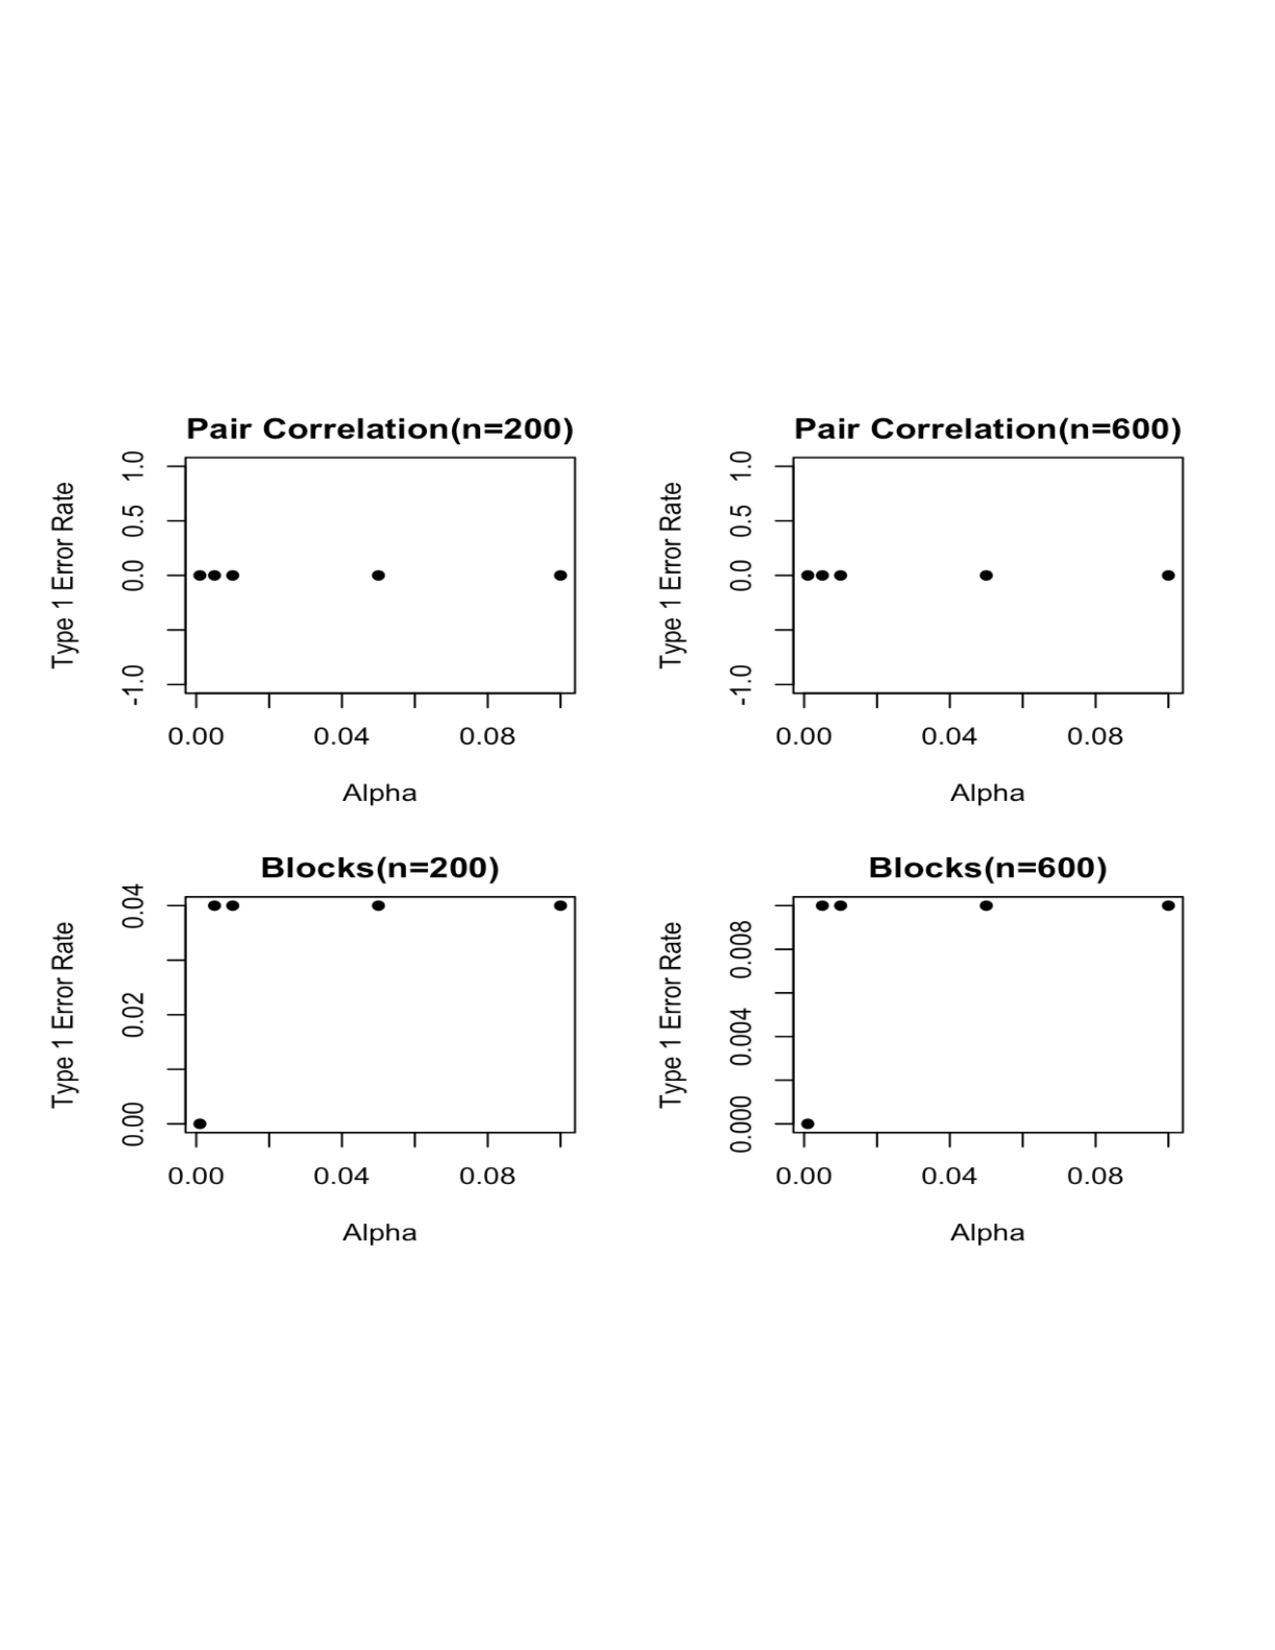
\includegraphics[width=10cm]{Powergraph1nonparam.pdf}
\caption{Graph of first four scenarios to calculate the power of a test}
\label{fig: Power Graphs 1}
\end{figure}

\begin{figure}[!hb]
\centering
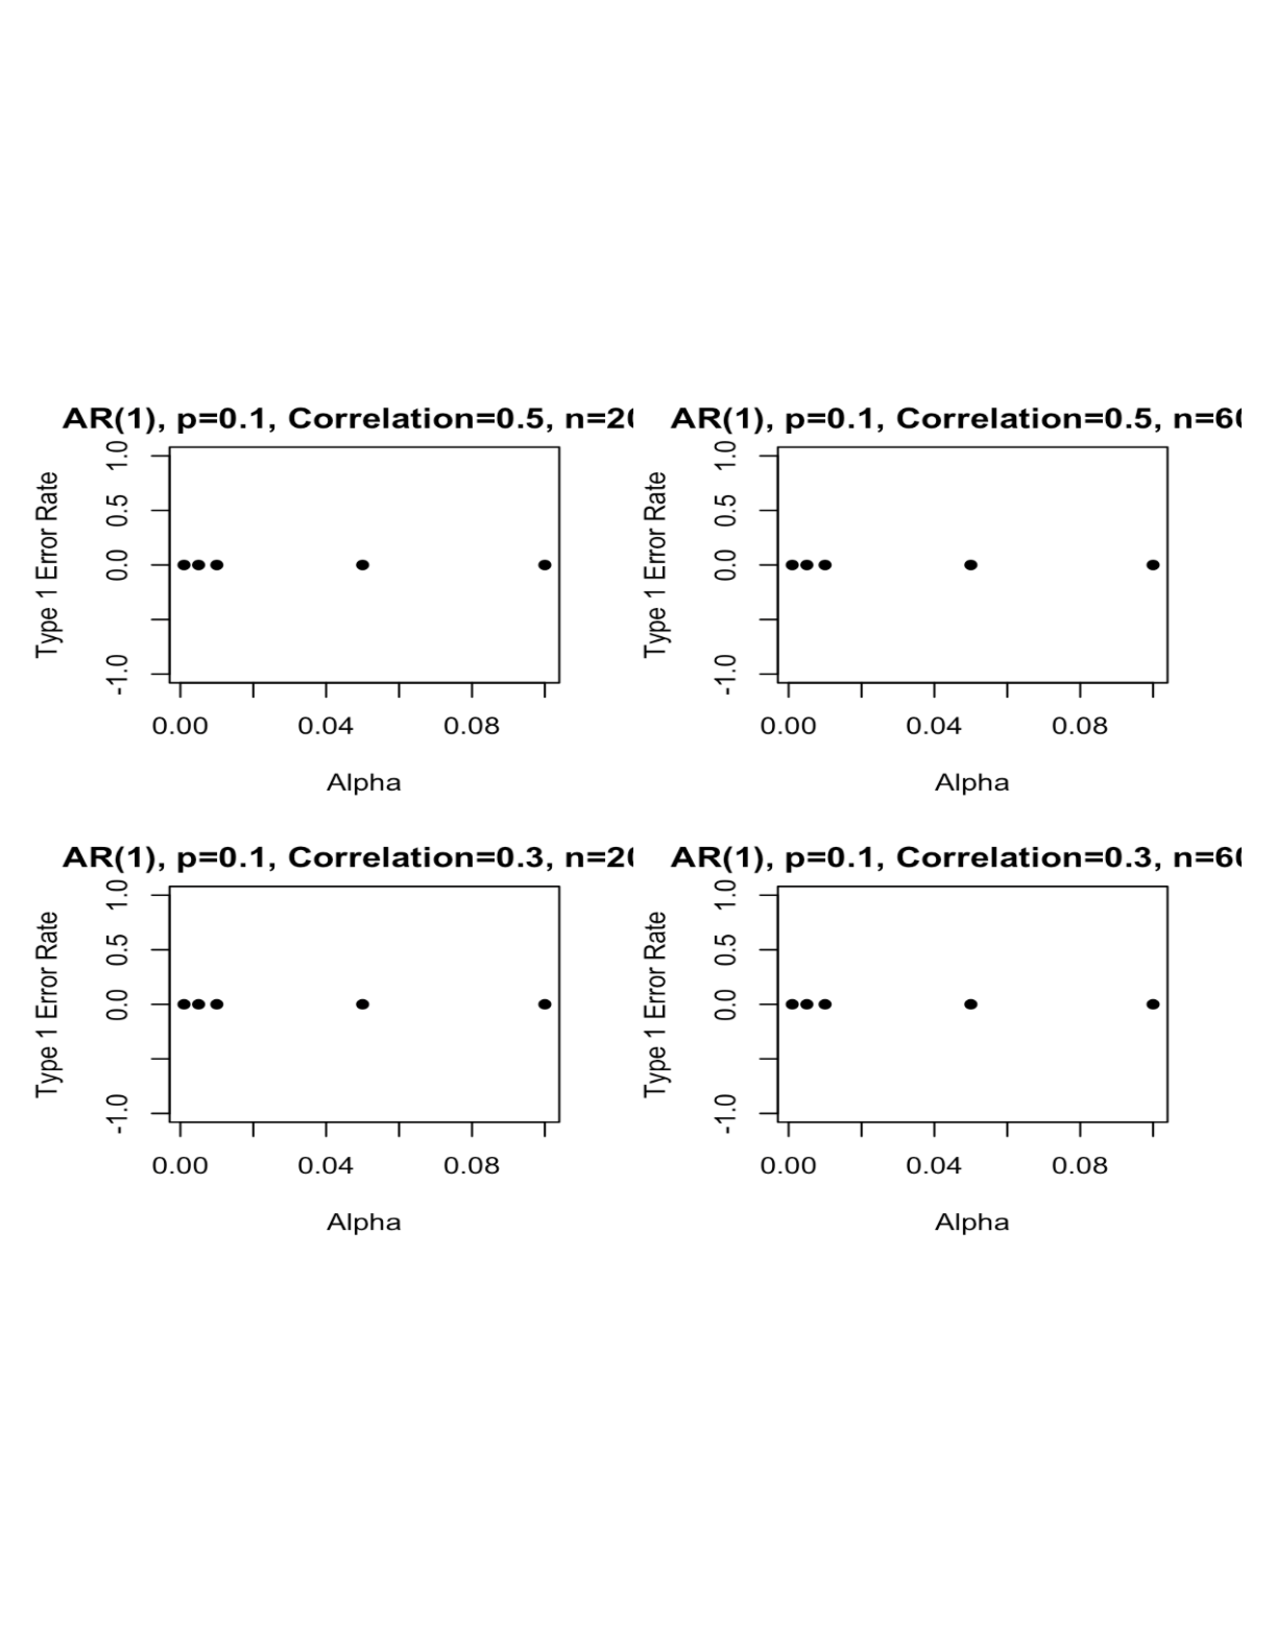
\includegraphics[width=10cm]{Powergraph2nonparam.pdf}
\caption{Graph of second four scenarios to calculate the power of a test}
\label{fig: Power Graphs 2}
\end{figure}

\begin{figure}[!hb]
\centering
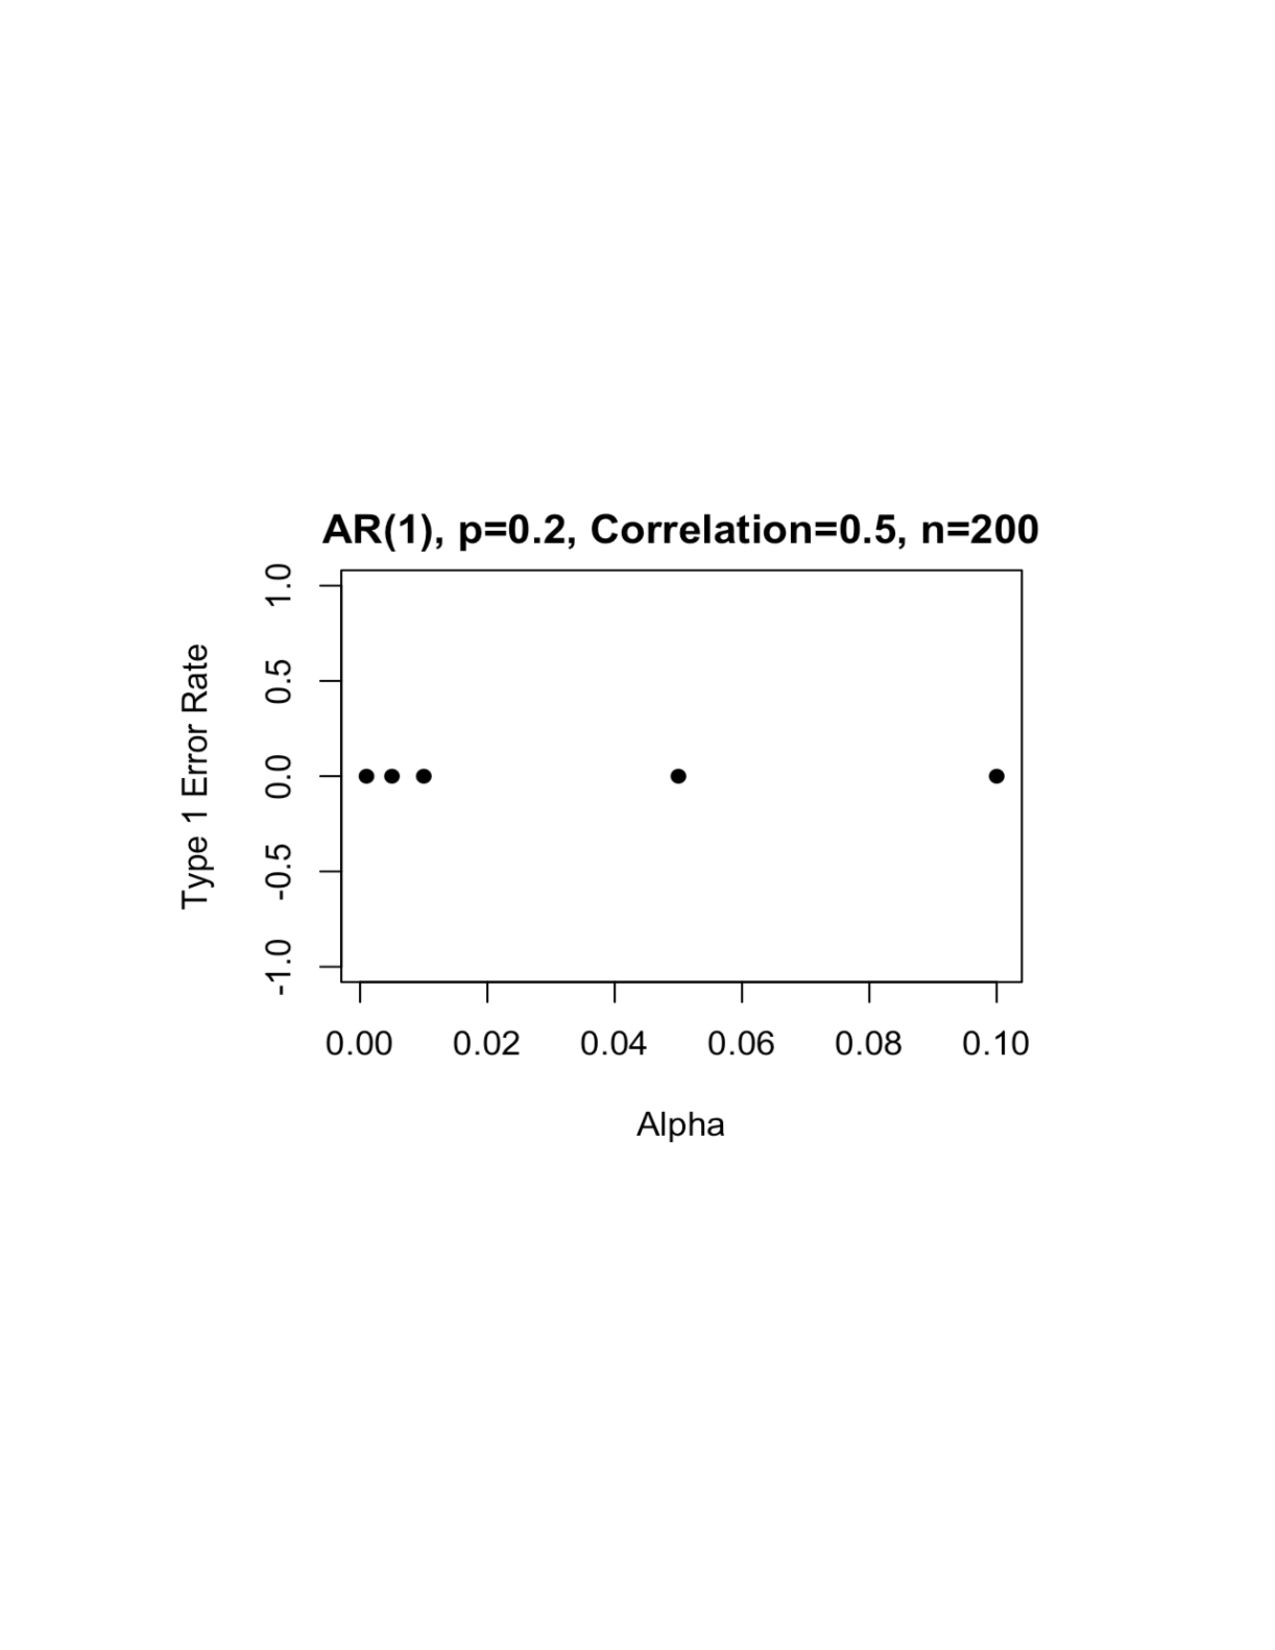
\includegraphics[width=10cm]{Powergraph3nonparam.pdf}
\caption{Graph of second to last scenario to calculate the power of a test}
\label{fig: Power Graphs 3}
\end{figure}

\begin{figure}[!hb]
\centering
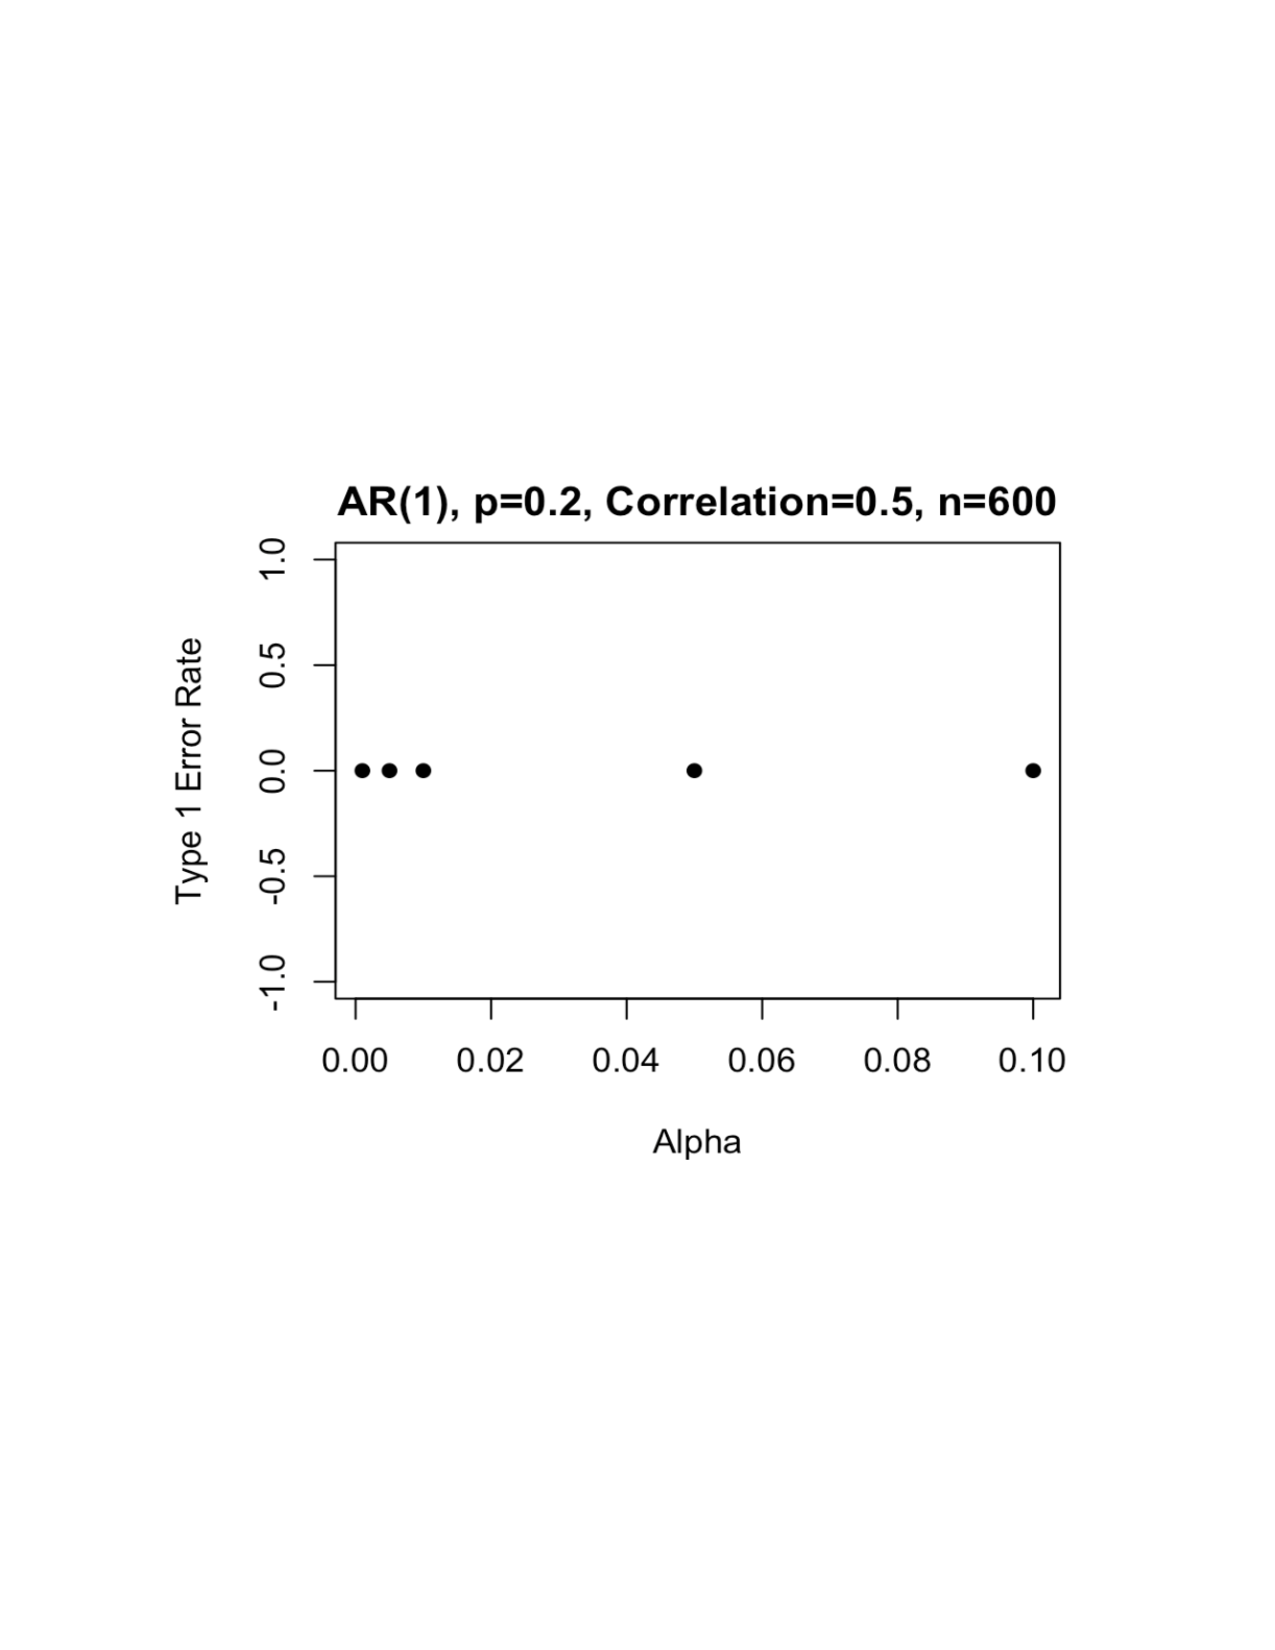
\includegraphics[width=10cm]{Powergraph4nonparam.pdf}
\caption{Graph of the last scenario to calculate the power of a test}
\label{fig: Power Graphs 4}
\end{figure}

\begin{figure}[!hb]
\centering
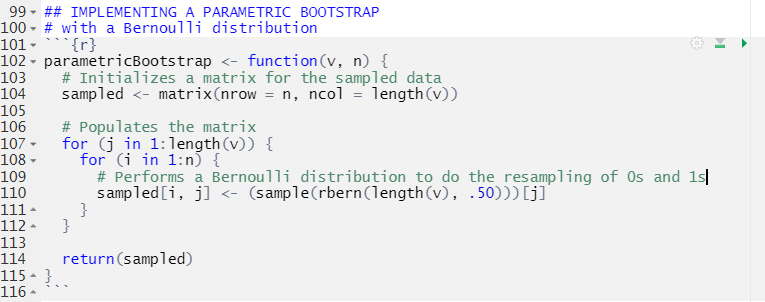
\includegraphics[width=10cm]{ParametricBootstrapCode.png}
\caption{Code to perform a Parametric Resampling on the data given}
\label{fig: Parametric Bootstrap Code}
\end{figure}

\begin{figure}[!hb]
\centering
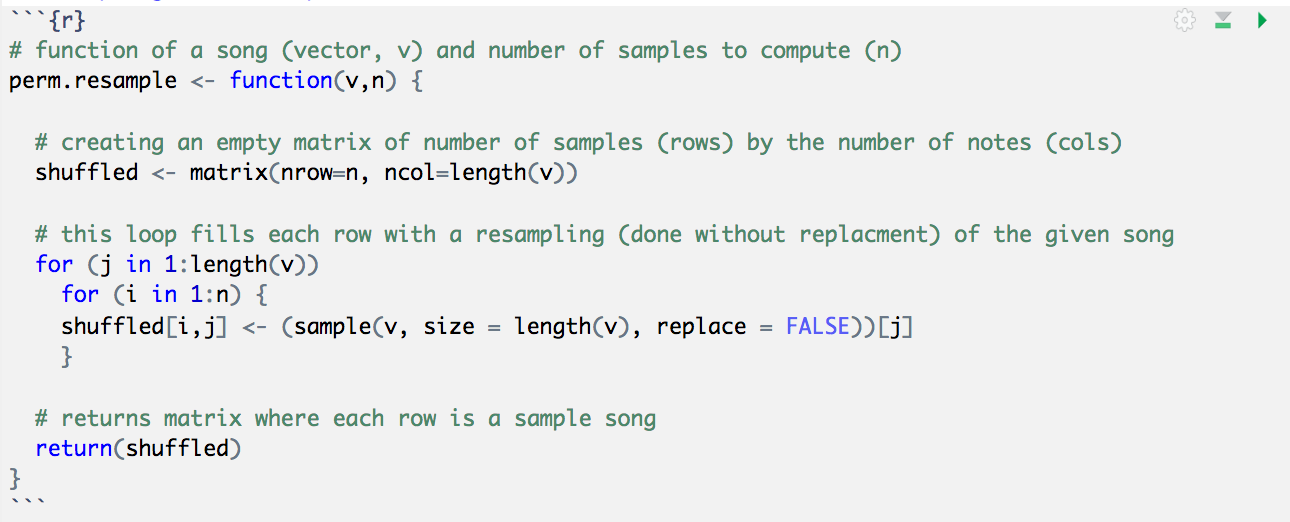
\includegraphics[width=10cm]{PermutationResamplingCode.png}
\caption{Code to perform Permutation Resampling on a vector of a song}
\label{fig: Permutation Resampling Code}
\end{figure}

\begin{figure}[!hb]
\centering
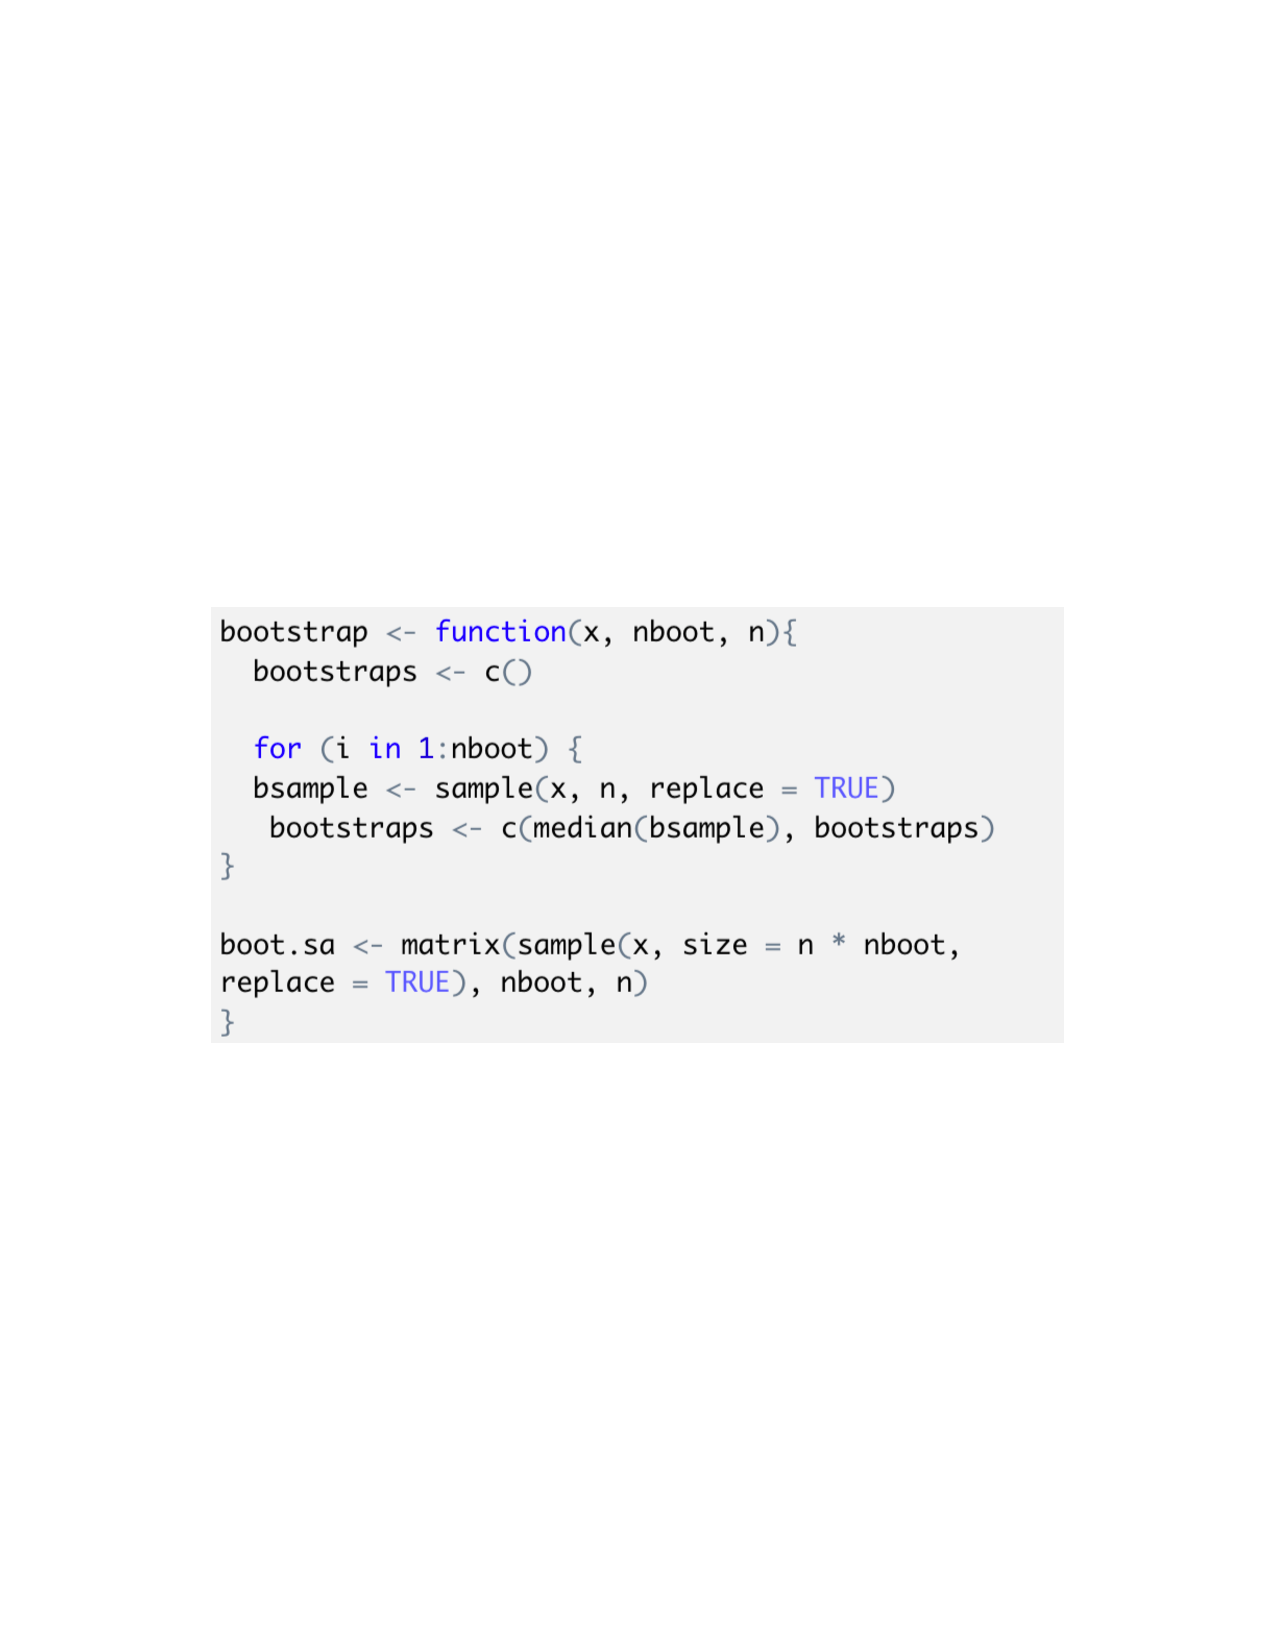
\includegraphics[width=10cm]{BootstrapCode.pdf}
\caption{Code to perform Nonparametric Bootstrap Resampling on a vector of a song}
\label{fig: Permutation Resampling Code}
\end{figure}

\begin{figure}[!hb]
\centering
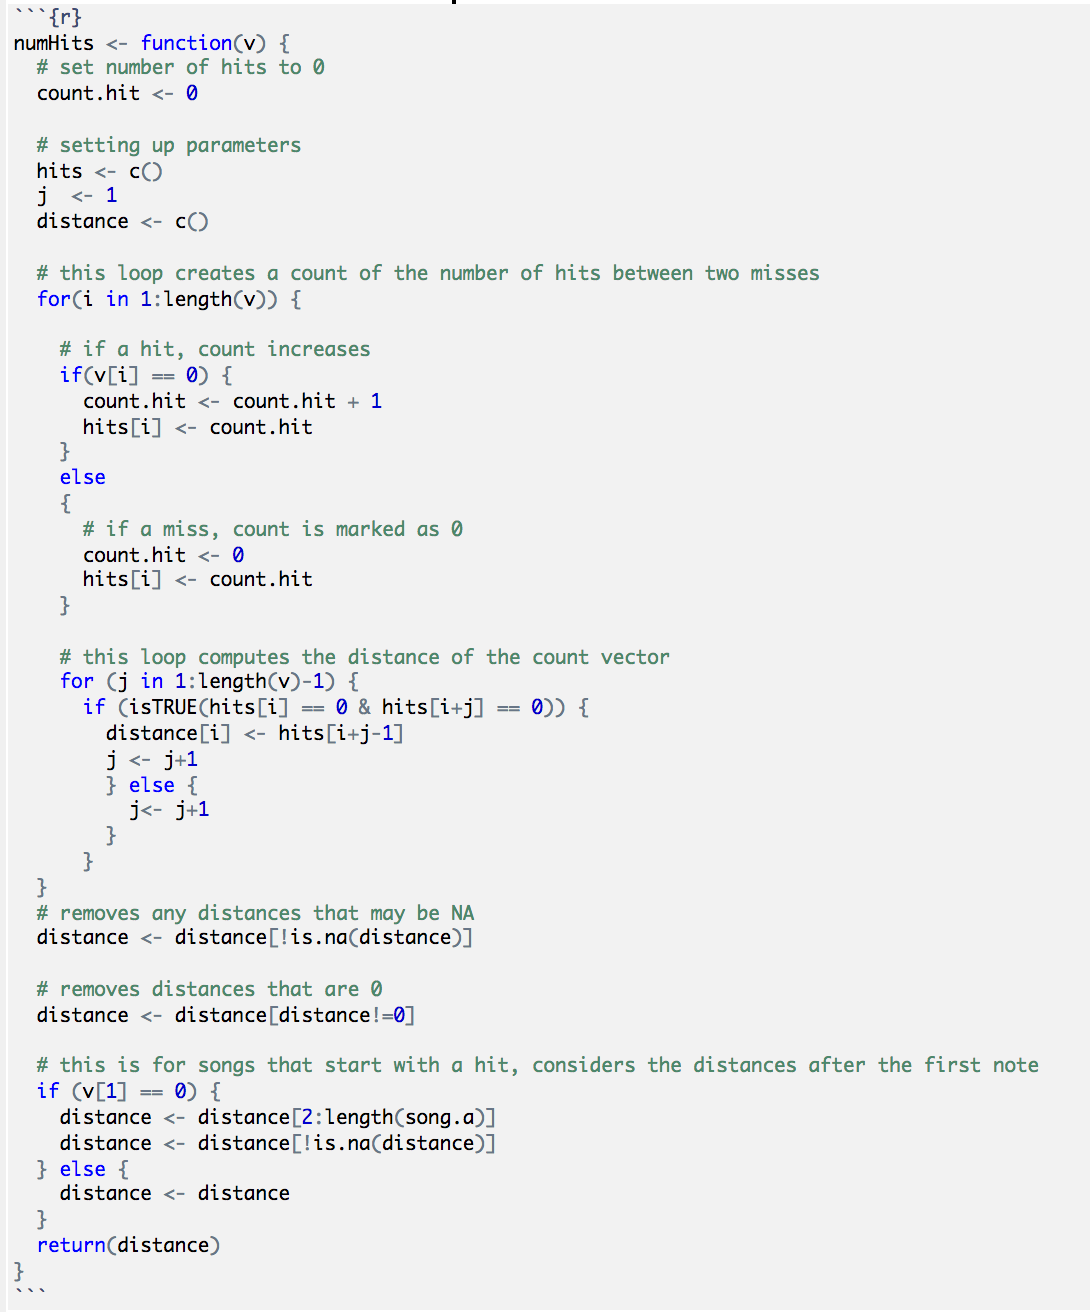
\includegraphics[width=10cm]{DistancesCode.png}
\caption{Code to compute the distances on a given vector of a song}
\label{fig: Distances Code}
\end{figure}

\begin{figure}[!hb]
\centering
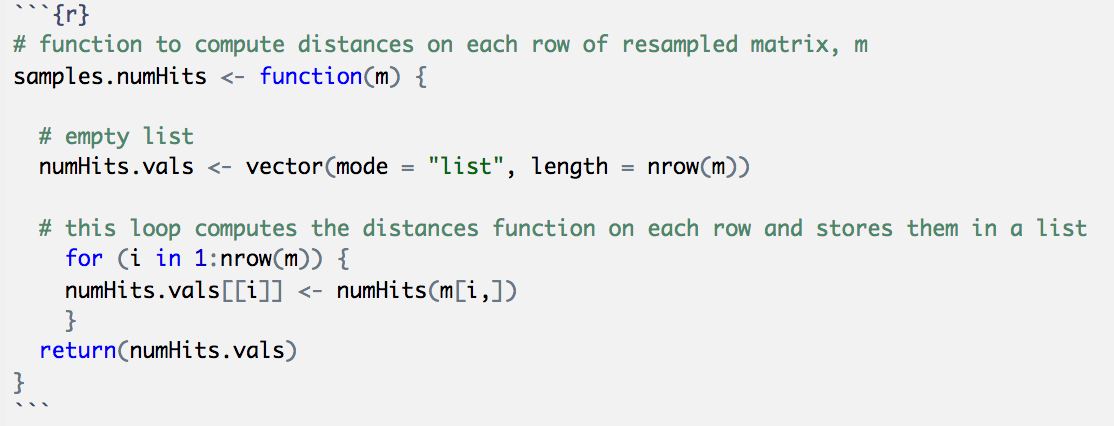
\includegraphics[width=10cm]{DistanceCodeforSamples.png}
\caption{Code to compute the distances on a given matrix of songs (all samples)}
\label{fig: Distances Code for Samples}
\end{figure}

\begin{figure}[!hb]
\centering
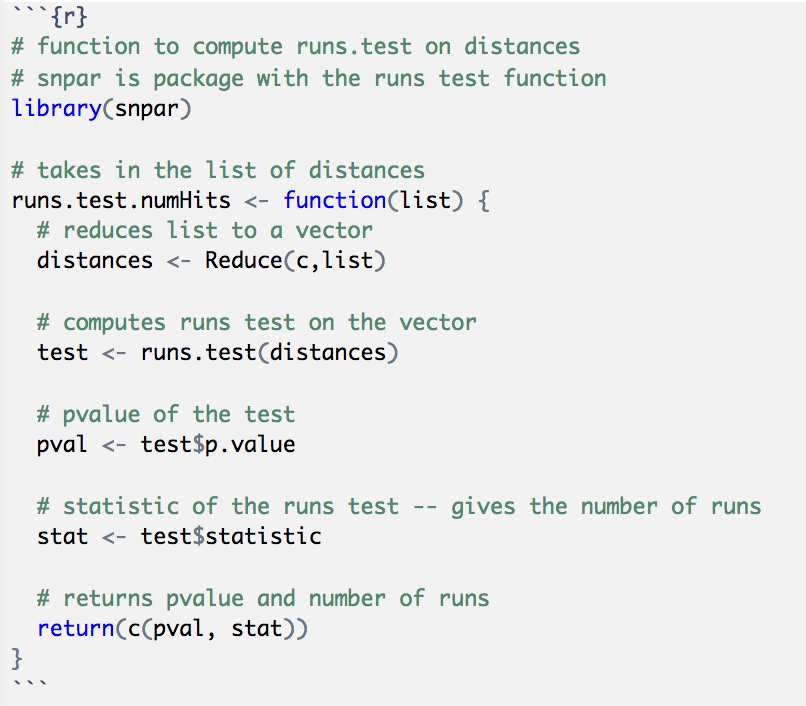
\includegraphics[width=10cm]{RunsTestforSamples.png}
\caption{Code to compute the runs test on all samples}
\label{fig: Runs Test Code for Samples}
\end{figure}

\begin{figure}[!hb]
\centering
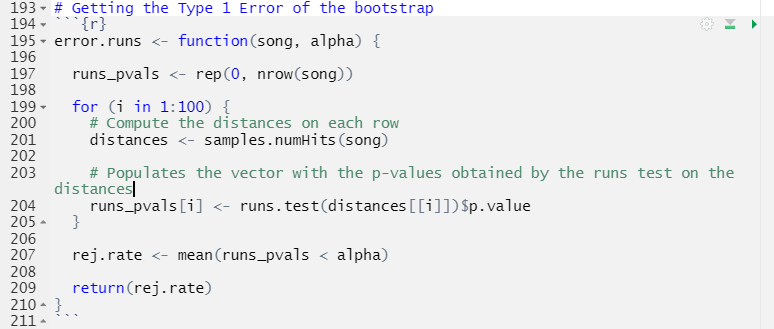
\includegraphics[width=10cm]{Type1ErrCode.png}
\caption{Code to get the Type 1 error of the inputted song}
\label{fig: Type 1 Error Code}
\end{figure}

\begin{figure}[!hb]
\centering
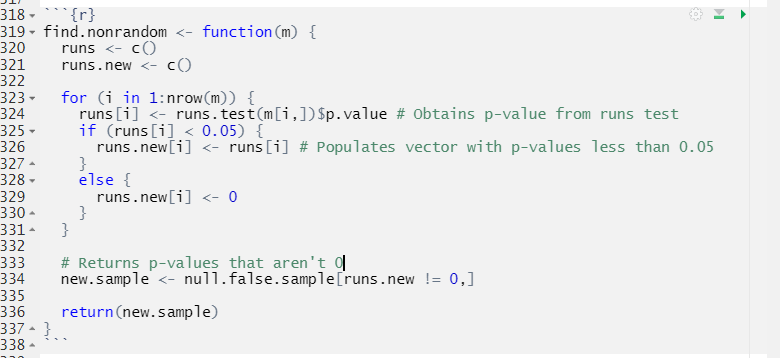
\includegraphics[width=10cm]{FindNonRandomCode.png}
\caption{Code finds the songs that are not random within the matrix}
\label{fig: Find Nonrandom Songs Code}
\end{figure}

\begin{figure}[!hb]
\centering
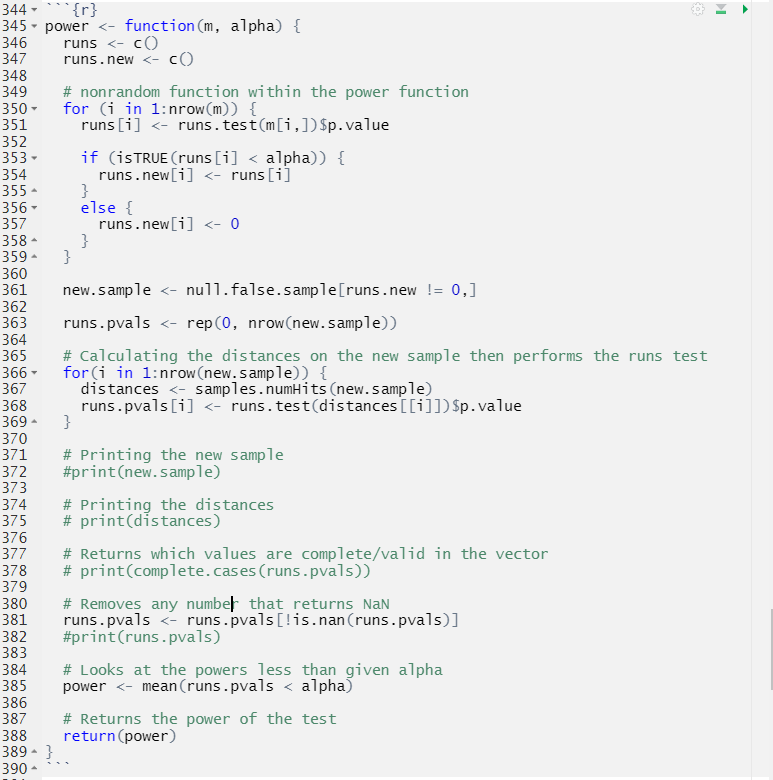
\includegraphics[width=10cm]{PowerCode.png}
\caption{Calculates the power of the test being performed on the song}
\label{fig: Power Code}
\end{figure}

\pagebreak

\section{PERSONAL REFLECTIONS}
\subsection{Brianna Cirillo}
This course has truly taught me a lot about R. I have coded things in this class that I could have never imagined doing in my life. I have learned a lot about the way that I should code as well. I always coded the same way that I do math, I sit down and just push through it. I have learned that it is more of a process. You need to start and when you get stuck give yourself a break and come back to it with a fresh mind. I have seen that research is hard work and there is a lot that goes into it. There is so much background that needs to be done before getting to any actual statistic or computing. I have also realized that getting it right doesn't really exist, and as someone great has said plenty of time, "celebrate the little victories". It is most definitely a process. I was very surprised at how much I knew about statistics and R. I definitely downplay my knowledge and this course showed me that I know more than I think. The impact it has made on my future is that I probably will not go in the research direction. This class gave me a lot of anxiety about if I was on the right path or doing the right thing, which goes back to me doubting my skills and knowledge. 

This course taught me that I definitely appreciate either complete guidance or complete control. I like to be able to either just complete an assignment or figure out what I need to do and do it the way that most makes sense in my head. I have realized that when I am extremely frustrated I tend to walk away and come back to it later. But, the stress about not knowing how to fix it makes me think about it constantly until I figure it out. I definitely doubt myself more than I should, and when I am extremely stressed I doubt myself more. I think I work well with others, I love that we can throw ideas off of each other. Since this class was pretty diverse in major and skill level, I think we all brought something different to the table. The group part of this class was so great, because it  allowed us to grow together.

To make this course better next time, I think we should go over the things we were reading about as a class. Most of the time, I felt like I understood but not completely. This definitely showed when we started doing the project and it was time to apply everything. I also think it may be beneficial to do the readings and then work on that part  of the project. I felt a little confused on some topics when we started doing them, just because it had been a while since we learned about it. I also think it would be beneficial if the layout was similar to consulting. If we had one assignment due every work that we got to work on for one class period, and then present the next class time. Overall, this class was an amazing experience and truly taught me a lot. It was a lot of work, but so worth it in the end. I definitely feel like I have grown as a person and a statistician.

\subsection{Samantha Colucci}
This course was extremely beneficial for me in many different aspects. Prior to this semester I had little background in advanced statistics, only having taken Prob&Stats II and having some practice from Consulting last semester. However, this class I learned a lot about the methodology behind statistical methods including how they are formed and how to form one on our own. I learned that when researching new methods, I work best with examples that are well explained and examples that I can recreate on my own. I also learned that it is necessary to learn a new topic one step at a time, rather than all at once, and to start with simpler examples. Though we ran into a lot of issues, I learned that this was okay and that it was actually a part of the process, regardless of how frustrating it can be. I was surprised with how much I actually enjoyed this process of trial and error because of how frustrating it was to me. However, once I accepted that I might not be able to figure everything out all at once, it became a more enjoyable process that almost became like a game. Due to this new found interest I will definitely want to experience more of this and will hopefully be able to do this more in my future. This course taught me a lot about how I learn and what works best for me when learning topics from readings and code. I feel that with a good combination of the two, I am able to grasp a new topic fairly well, and I can fully grasp it with some examples. A major thing I learned about myself is that I have a need to figure things out, and when I can’t I usually won’t stop working at it until I can. This happened many times during this research when I was trying to figure out how to write a new code or how to modify our method. I also learned that I enjoy working with other people because I like bouncing ideas off of others and hearing their ideas to see if it changes mine in any way. My group was a great to have when doing this project because everyone was helpful and was able to contribute a lot to the research. I also feel that me and my group both had a growth of self-confidence when dealing with this research, because as the semester continued we, most of the time, had a better and better grasp on what we needed to do. To improve the course, I would suggest discussing in detail the readings and assignments due in the beginning of the semester. I feel that if we had more of a discussion and went over the topics as a group the ideas would have stuck in my head better. I also feel that for some of the assignments for the research we needed more time to complete them and ask questions about what needed to be done. Other than that, I think this course was formatted really well and I loved how it was setup compared to other classes. This has definitely been one of my favorite classes that I have taken at Monmouth and I am grateful to have had this experience.


\subsection{Shannon Coyle}
From this course, I've definitely gained more knowledge about R Studio and how to perform functions, equations, and other features along with new statistics skills.  In previous courses, I understood the math behind confidence intervals and p-values, but this course truly helped me understand the application and importance of those two components.  It was different learning statistics to apply it to actual data as opposed to just doing the math for homework and tests to get a grade.  When researching, I learned that ideas are not going to work 100\% of the time and that is okay, trial-and-error is an integral part of research that everyone has to go through.  I was also able to learn more from my peers than from the professor because we have a different understanding of topics than a professor does.  I can confidently say that I have a better understanding of statistics after getting explanations from my peers instead of being taught on a whiteboard by someone who has somewhat mastered the topic.  Taking this class has made me more interested in the data science aspect of computer science, whereas, before this course I was on the fence about the crossover between coding and mathematics.  For my future, this course has given me another coding language that I can say that I understand as well as showing me the importance of data and computing.  

I definitely learned a lot about myself by taking this course - both good and bad attributes.  My patience could use some work when it comes to coding, when things would not work the way I wanted to it made me feel like a failure and I would give up.  I did learn that not even the best coders can get these things right the first time.  I also realized that I can work in groups and with whatever I do in my future, I will have to work with others in the technological world.  It was helpful to have Bri and Sam pick me up when I was down and help me understand any of the information that I was struggling to grasp.  They truly helped me with my stress and frustrations, but aside from that, I would take breaks if I found myself getting overly frustrated and remind myself that we were trying to do something that most people will not even attempt in their lifetime.  I was definitely surprised about how I was able to pick up some of the math concepts and then try to figure them out in R.  In the beginning of this class, I was convinced I should not be in it because I felt dumber than everyone else.  After this semester, I've realized that if I should not have been in the class, Dr. B would not have asked me to take it.  I've seen a lot of personal growth this semester, and I am really glad I was able to take this class.  

For the future of this course, I would have mini lessons about the homeworks we did in the beginning of the semester.  I was struggling to fully understand the material and I think having small lessons led by Dr. B would have helped me fully get the topic at hand.  I think the diaries are really important to the course, so I would keep those as well as presenting the homeworks to everyone else in the class.  I think that giving both assignments for the week at the same time would be beneficial if the days between classes aren't that spread out.  One of the hardest parts was finding time to do the second assignment for the week when we only had one full day to complete it.  Other than that, I truly loved this course and I am so glad I was able to take it.  


\end{document}